\documentclass[10pt,a4paper]{article}
\usepackage{hyperref, parskip}
\usepackage[super,sort&compress,comma]{natbib}
\usepackage{graphicx}
\usepackage{mathtools}
\usepackage{amssymb}
\usepackage{chemformula}
\title{"Computer modelling studies of new materials for lithium and sodium batteries" Data}
\author{Benedek Goldmann}

\begin{document}

\section{Lattice energies}

\begin{table}[h!]
  \begin{center}
    \caption{Lattice energies (LEs)}
    \label{tab:table1}
    \begin{tabular}{l|c|c|c|c}
      \textbf{Lattice} & \textbf{Calc. LE, eV} & \textbf{Exp. LE, eV} & \textbf{Lattice type} & \textbf{Space group}\\
      \hline
      \ch{Li3OCl} &-38.21 & - & antiperovskite & 221\\
      \ch{LiCl} & -8.59 & -8.96 & rocksalt & 225\\
      \ch{LiO2} & 29.02 & -29.45 & fluorite & 225\\
      \ch{Na3OCl} & -34.44 & - & antiperovskite & 221\\
      \ch{NaCl} & -8.09 & -8.19 & rocksalt & 225\\
      \ch{Na2O} & -26.30 & -25.68 & fluorite & 225\\
      \ch{MgCl2} & -26.52 & -26.33 & \ch{CdCl2} & 164\\
      \ch{MgO} & -41.16 & -39.29 & rocksalt & 225\\
      \ch{CaCl2} & -21.15 & -23.54 & rutile & 136\\
      \ch{CaO} & -35.88 & -35.25 & rocksalt & 225\\
      \ch{SrCl2} & -21.14 & -22.49 & fluorite & 225\\
      \ch{SrO} & -33.40 & -33.40 & rocksalt & 225\\
      \ch{BaCl2} & -20.16 & -21.44 & fluorite & 225\\
      \ch{BaO} & -31.20 & -31.65 & rocksalt & 225\\
    \end{tabular}
  \end{center}
\end{table}

Experimental values from David R. Lide (Editor-in-Chief): Handbook of Chemistry and Physics - 88th Edition, 2007-2008; pages 12-19 to 12-27.

\clearpage

\section{\ch{Li3OCl} data}

\begin{figure}[h!]
\centering
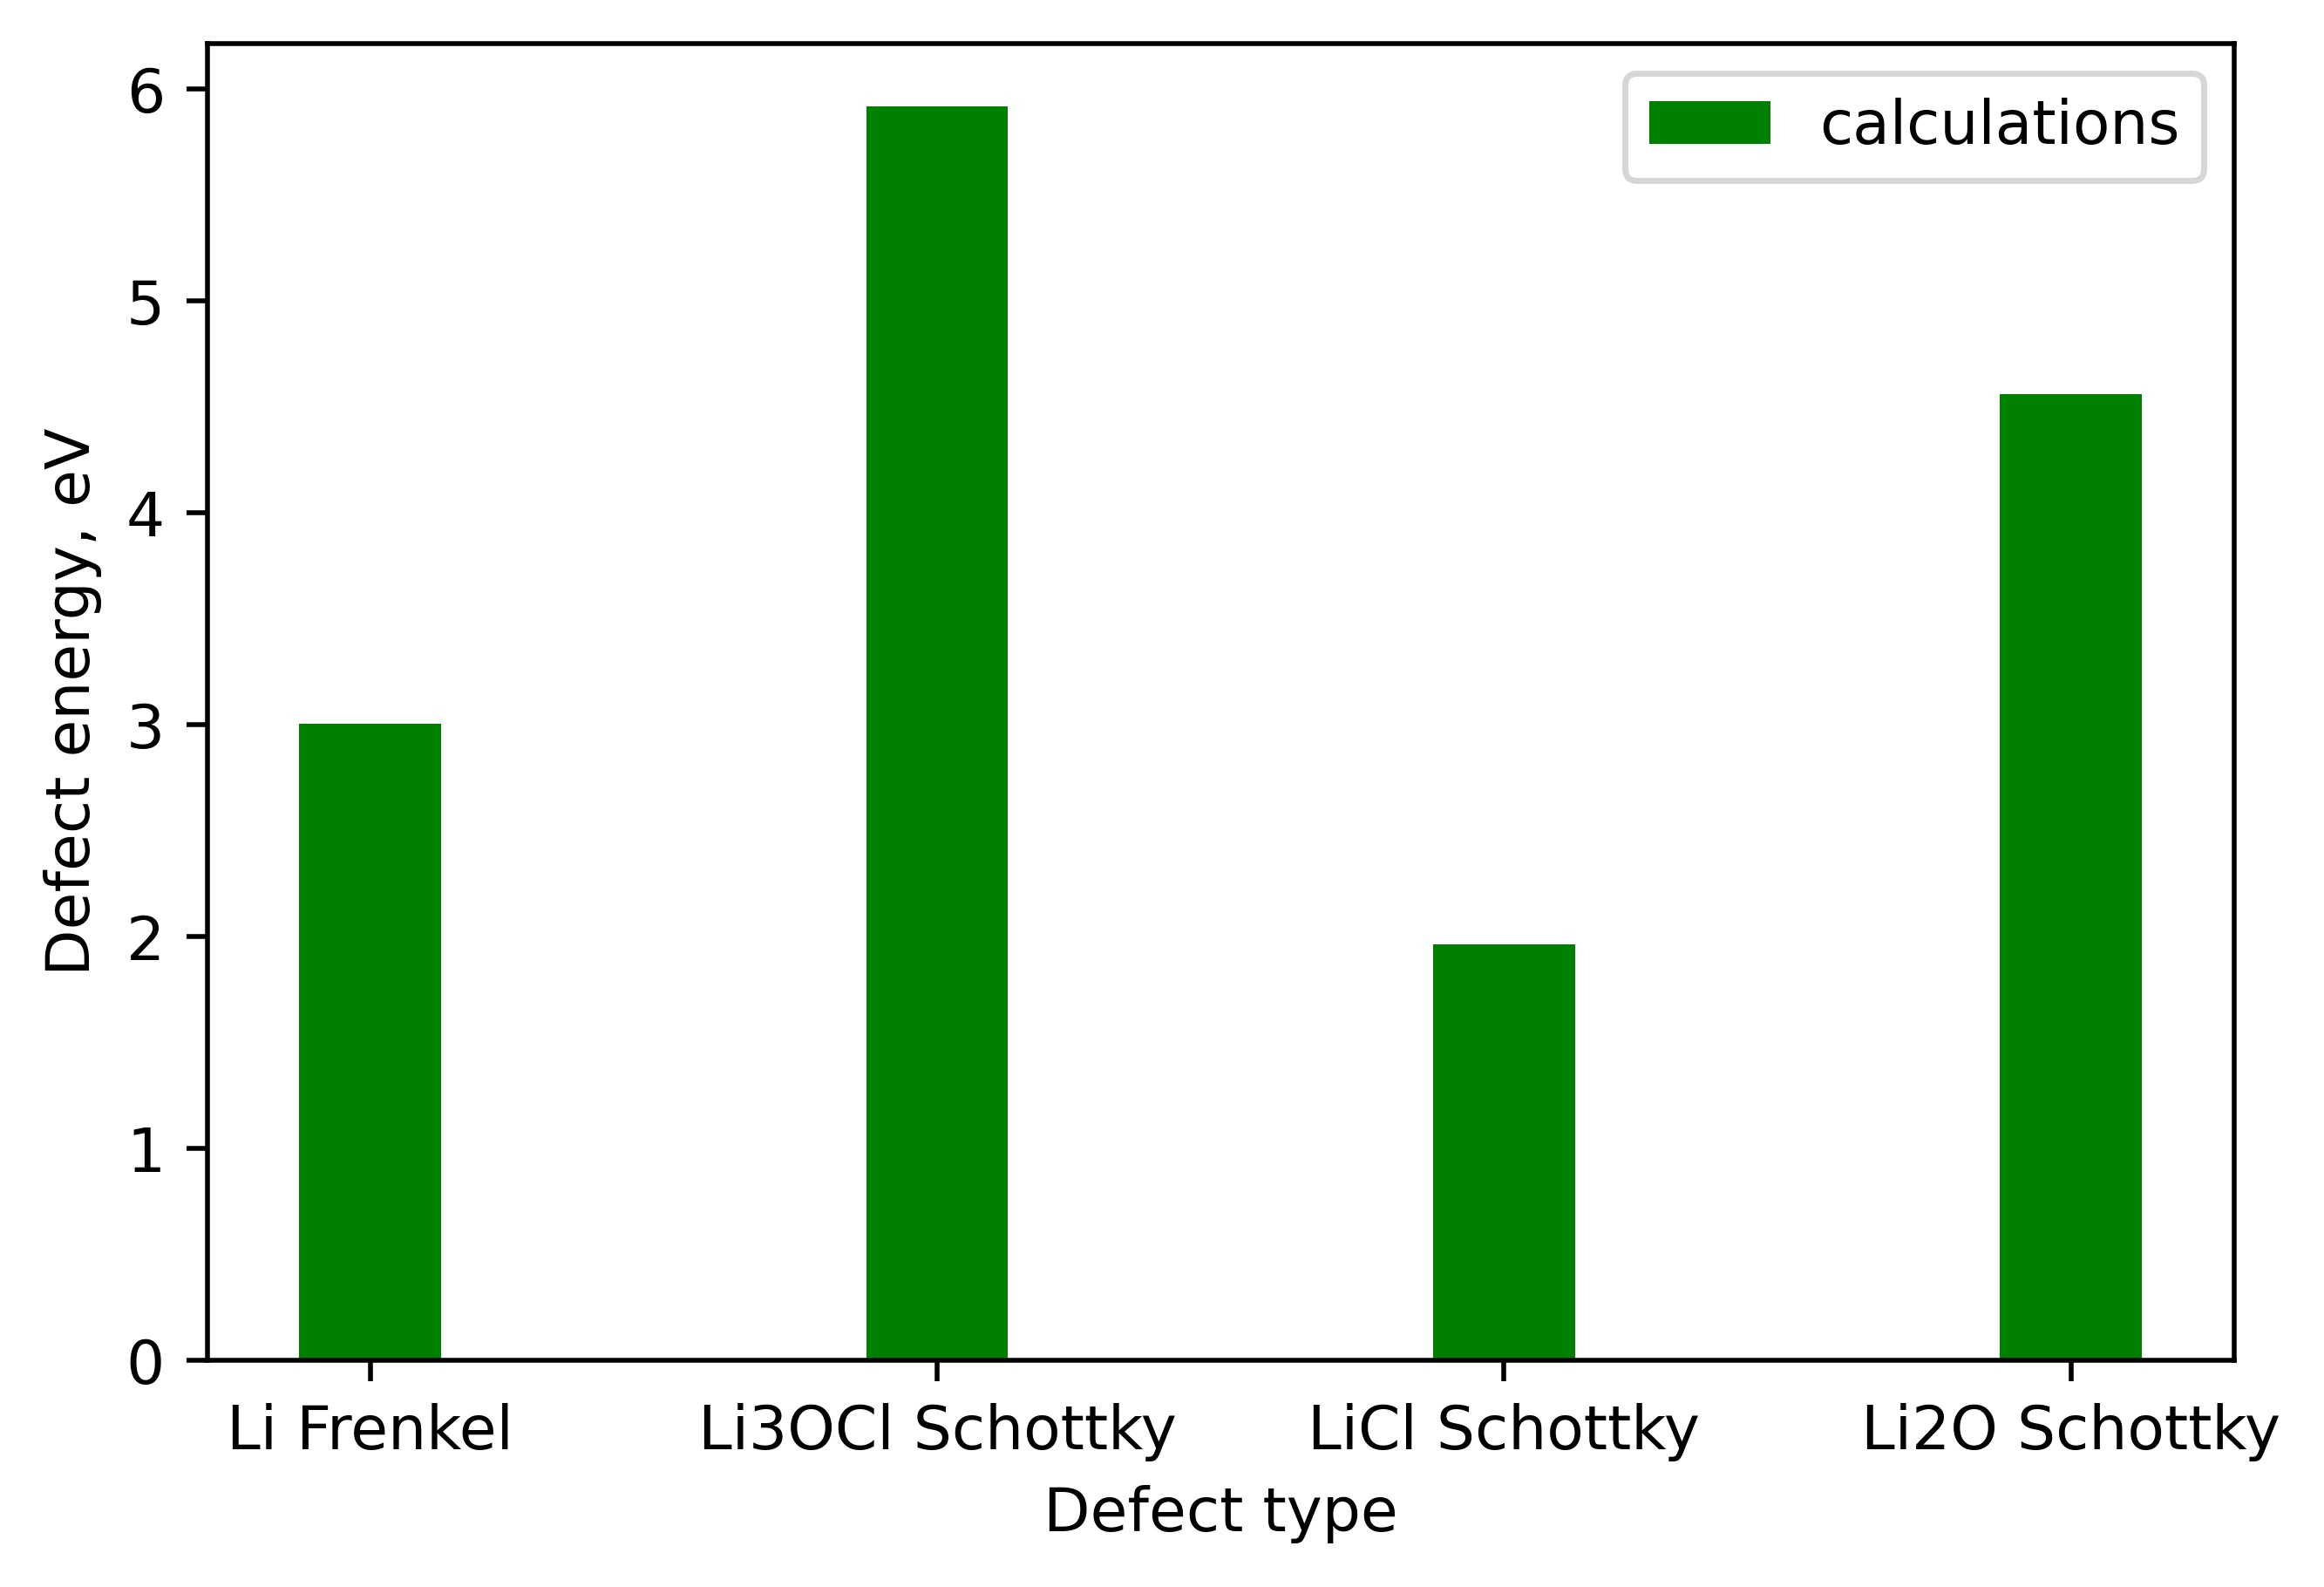
\includegraphics[width=10cm]{li3ocl_defects.jpg}
\caption{\label{li3ocl_defects.jpg} \ch{Li3OCl} defects}
\end{figure}

\begin{figure}[h!]
\centering
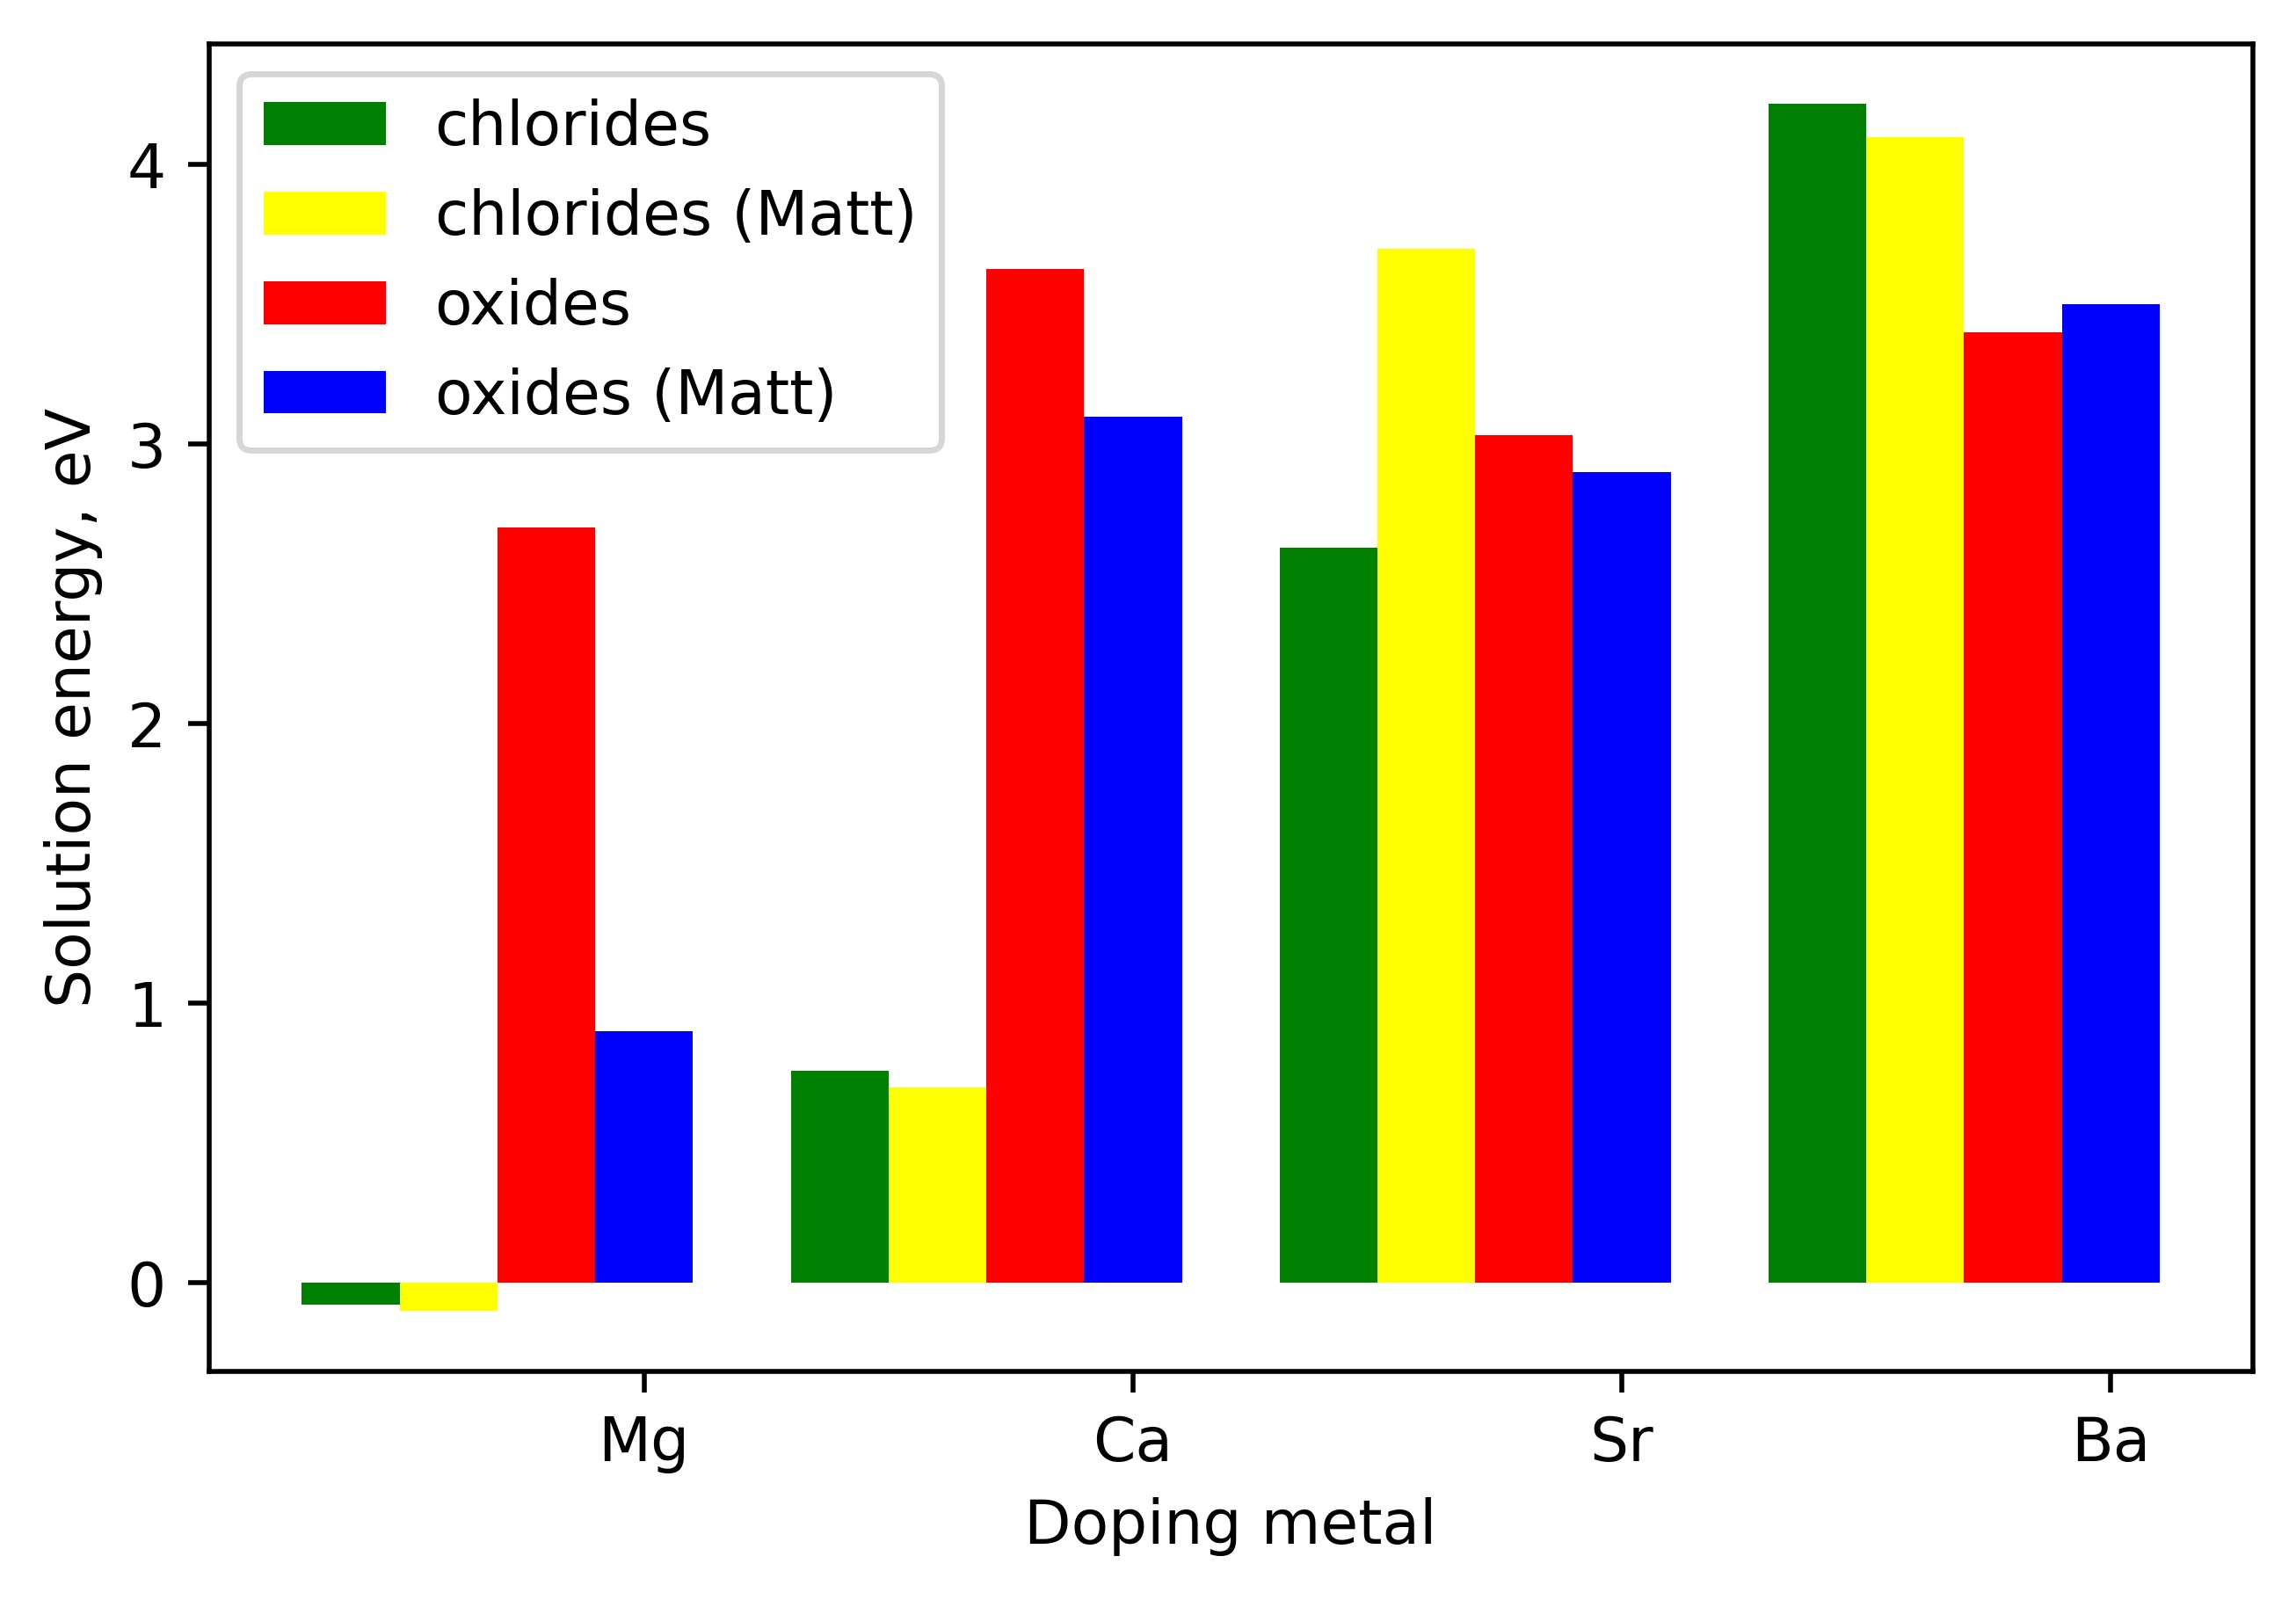
\includegraphics[width=10cm]{li3ocl_doping.jpg}
\caption{\label{li3ocl_doping.jpg} \ch{Li3OCl} doping}
\end{figure}

\begin{figure}[h]
\centering
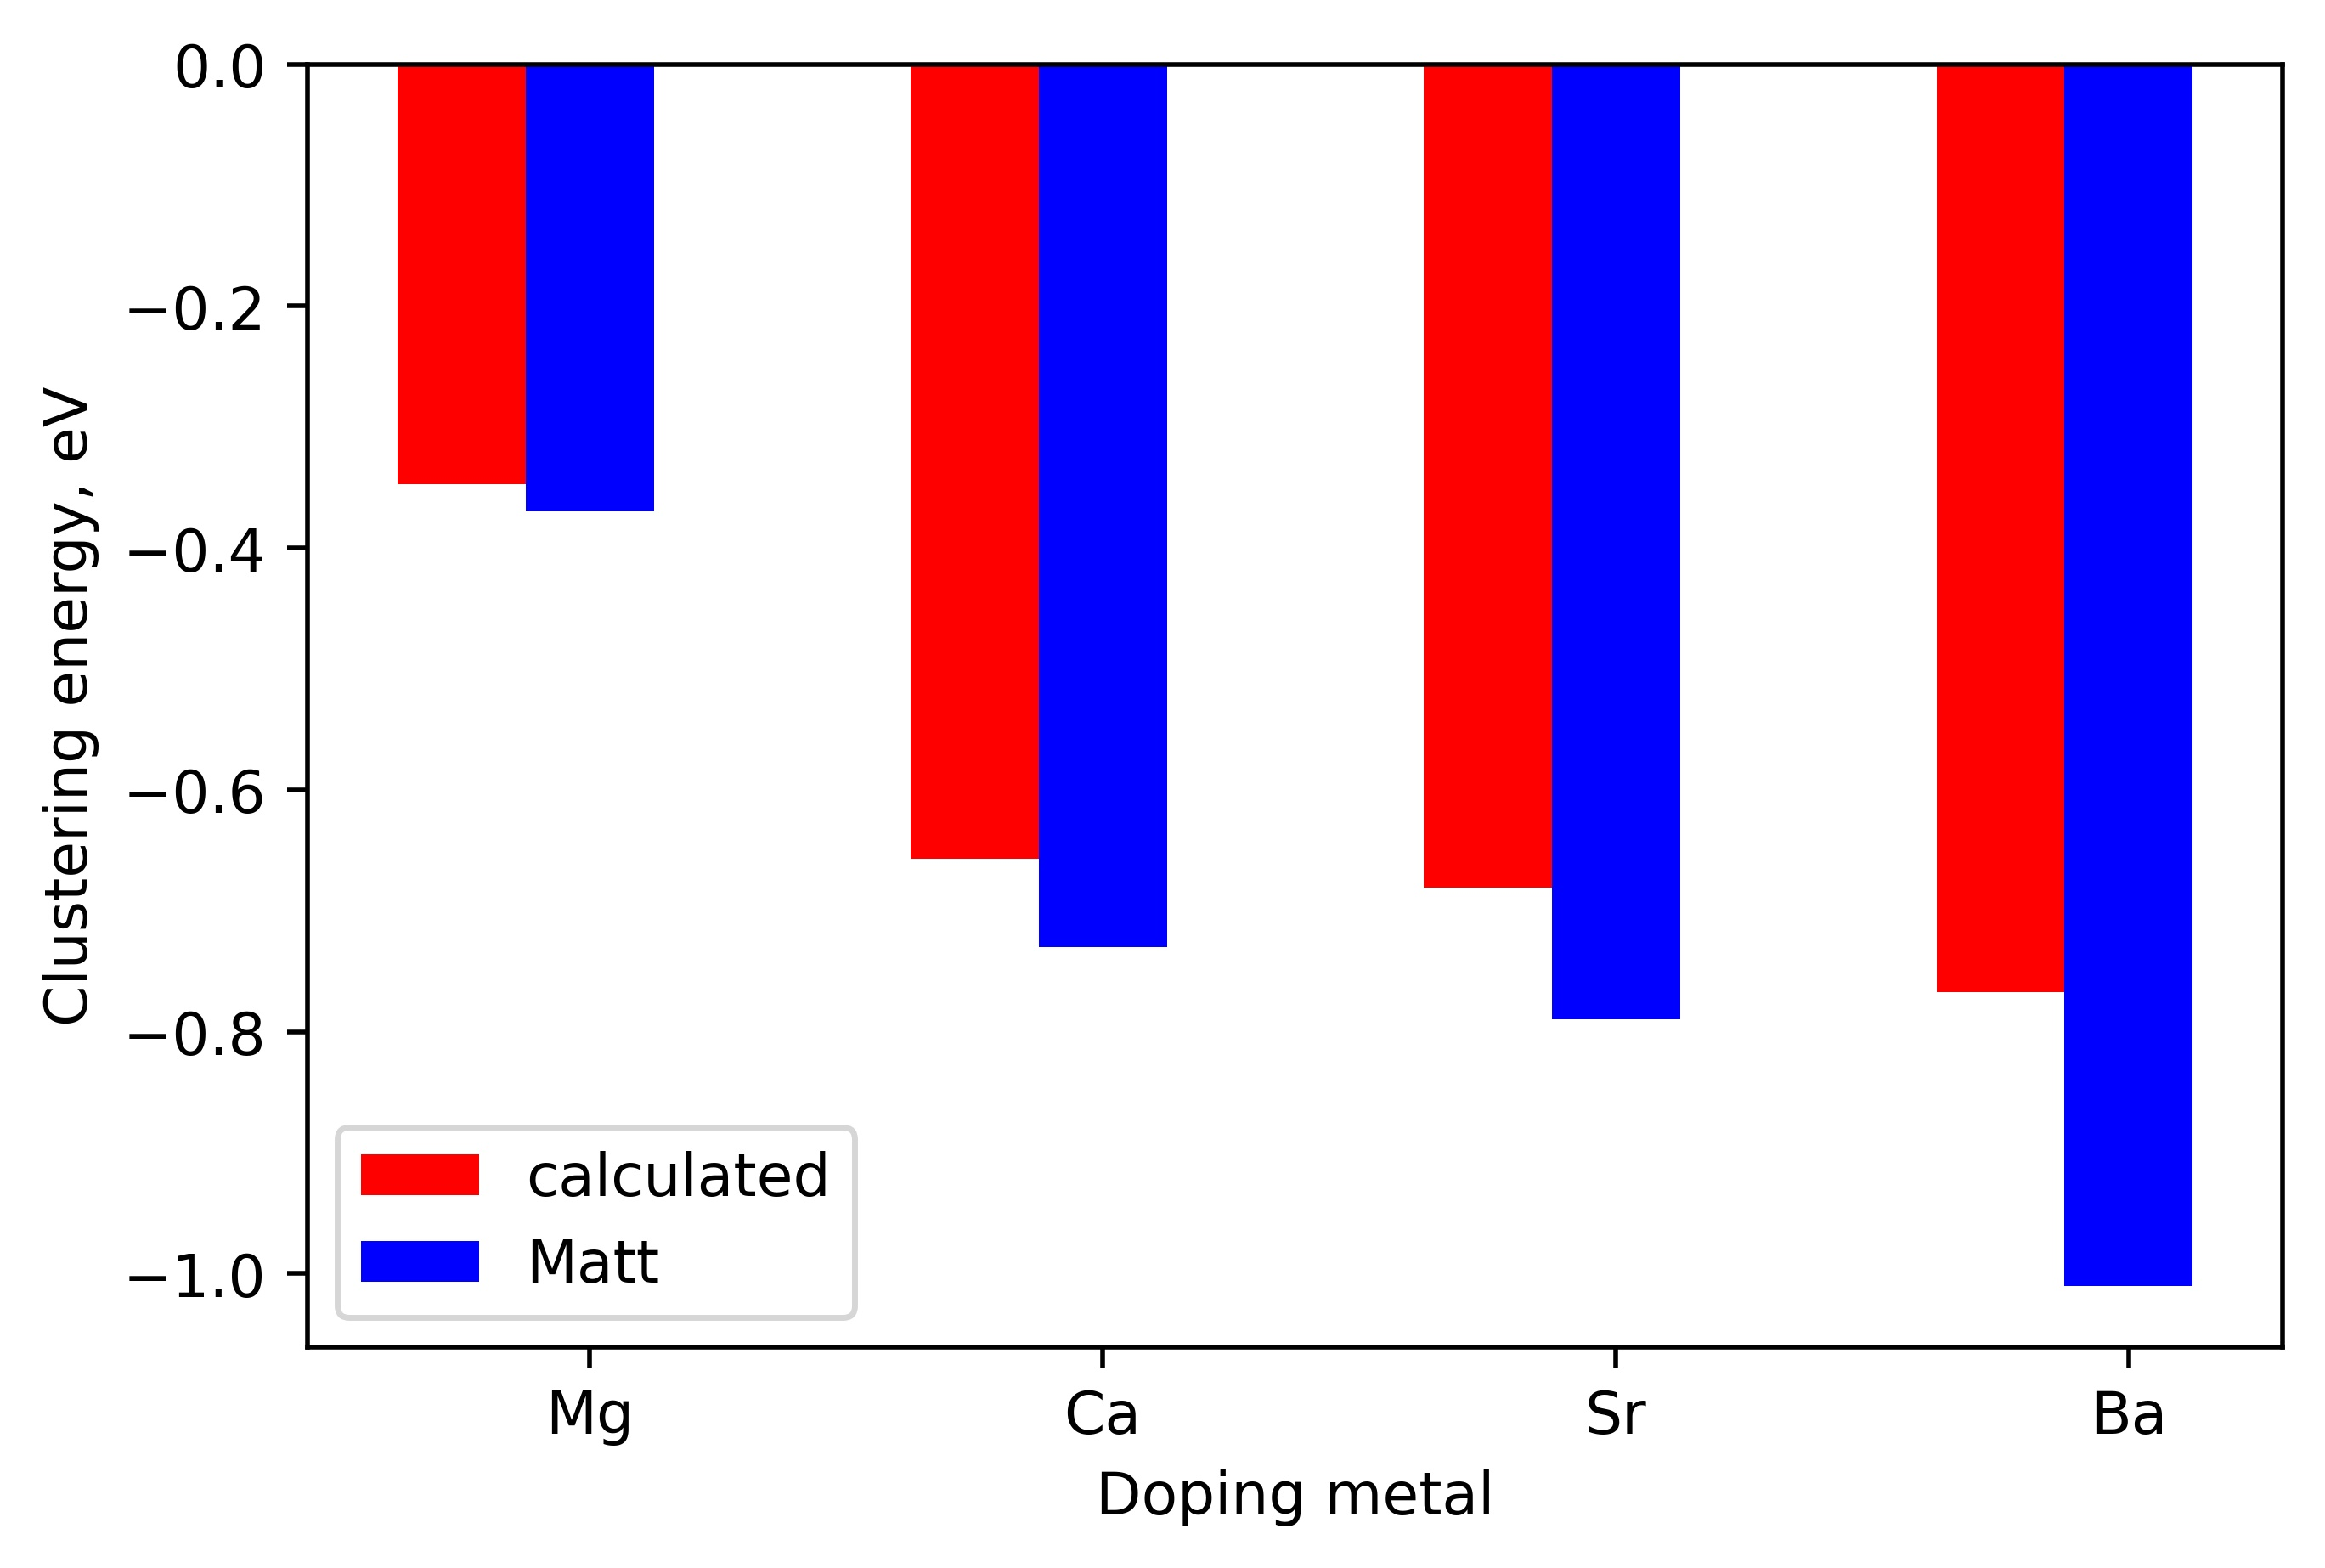
\includegraphics[width=10cm]{li3ocl_clustering.jpg}
\caption{\label{li3ocl_clustering.jpg} \ch{Li3OCl} clustering}
\end{figure}

\begin{figure}[h!]
\centering
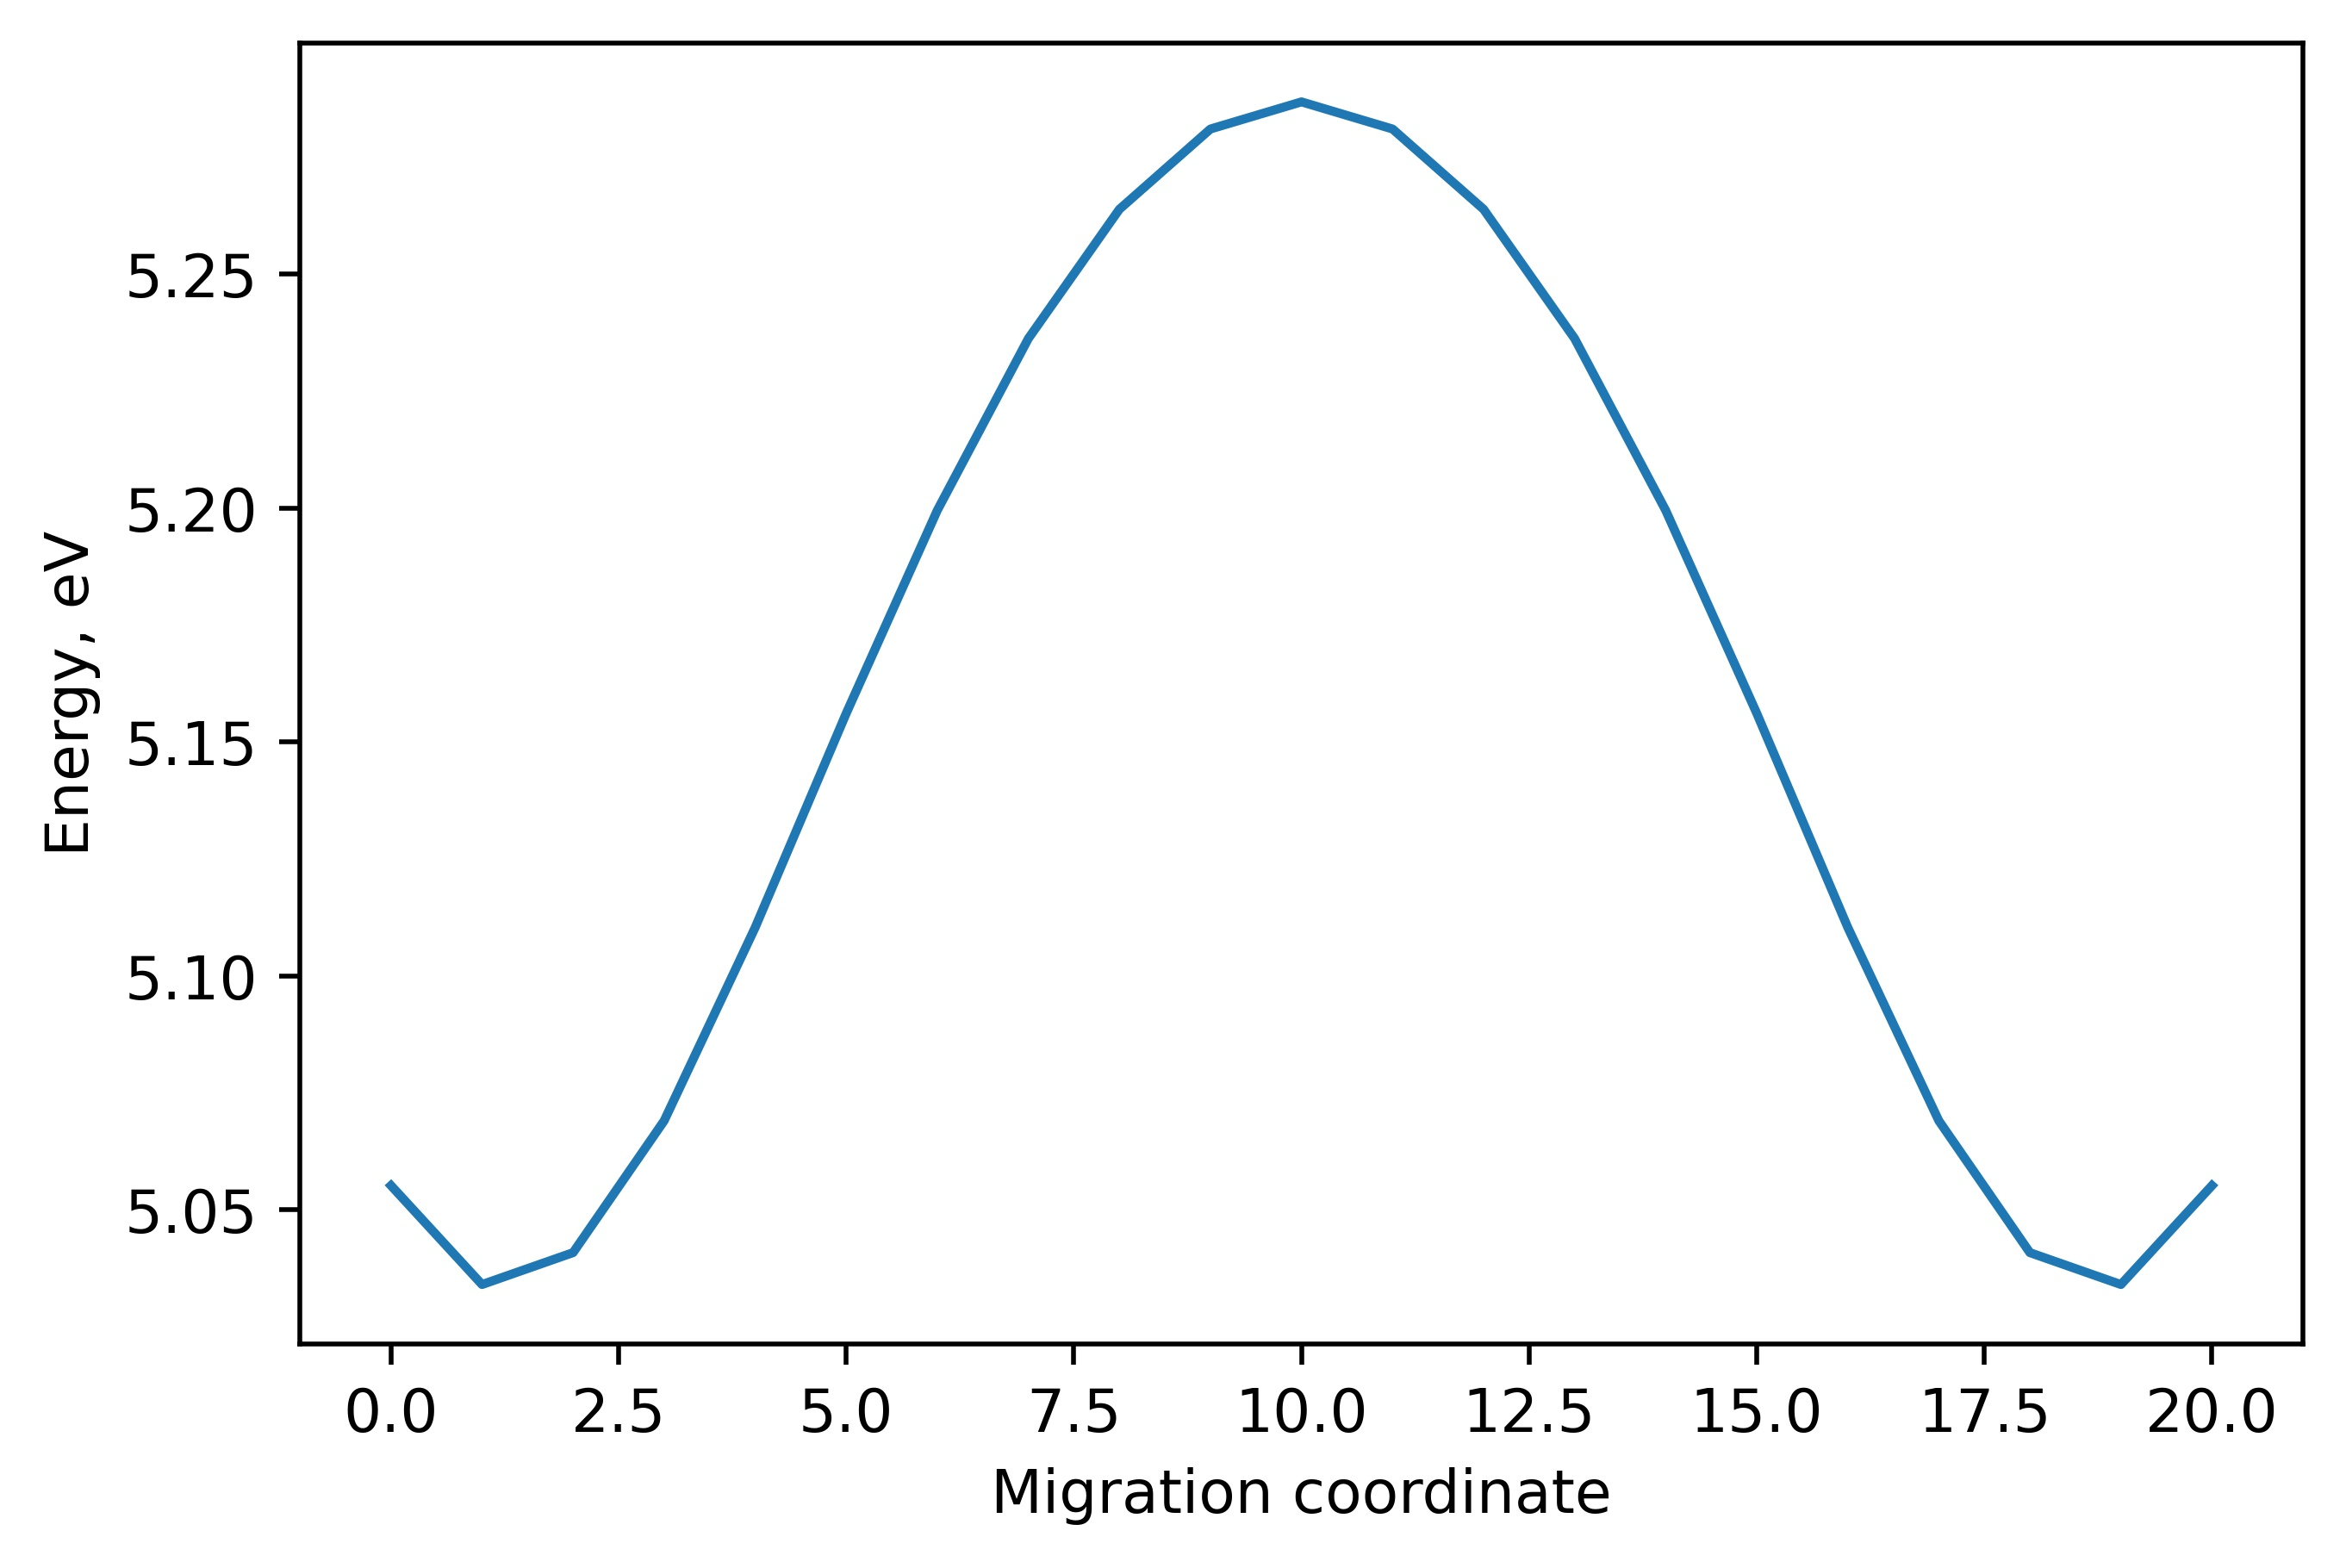
\includegraphics[width=10cm]{li3ocl_li_mig.jpg}
\caption{\label{li3ocl_li_mig.jpg} \ch{Li3OCl} lithium ion vacancy migration profile}
\end{figure}

\begin{figure}[h!]
\centering
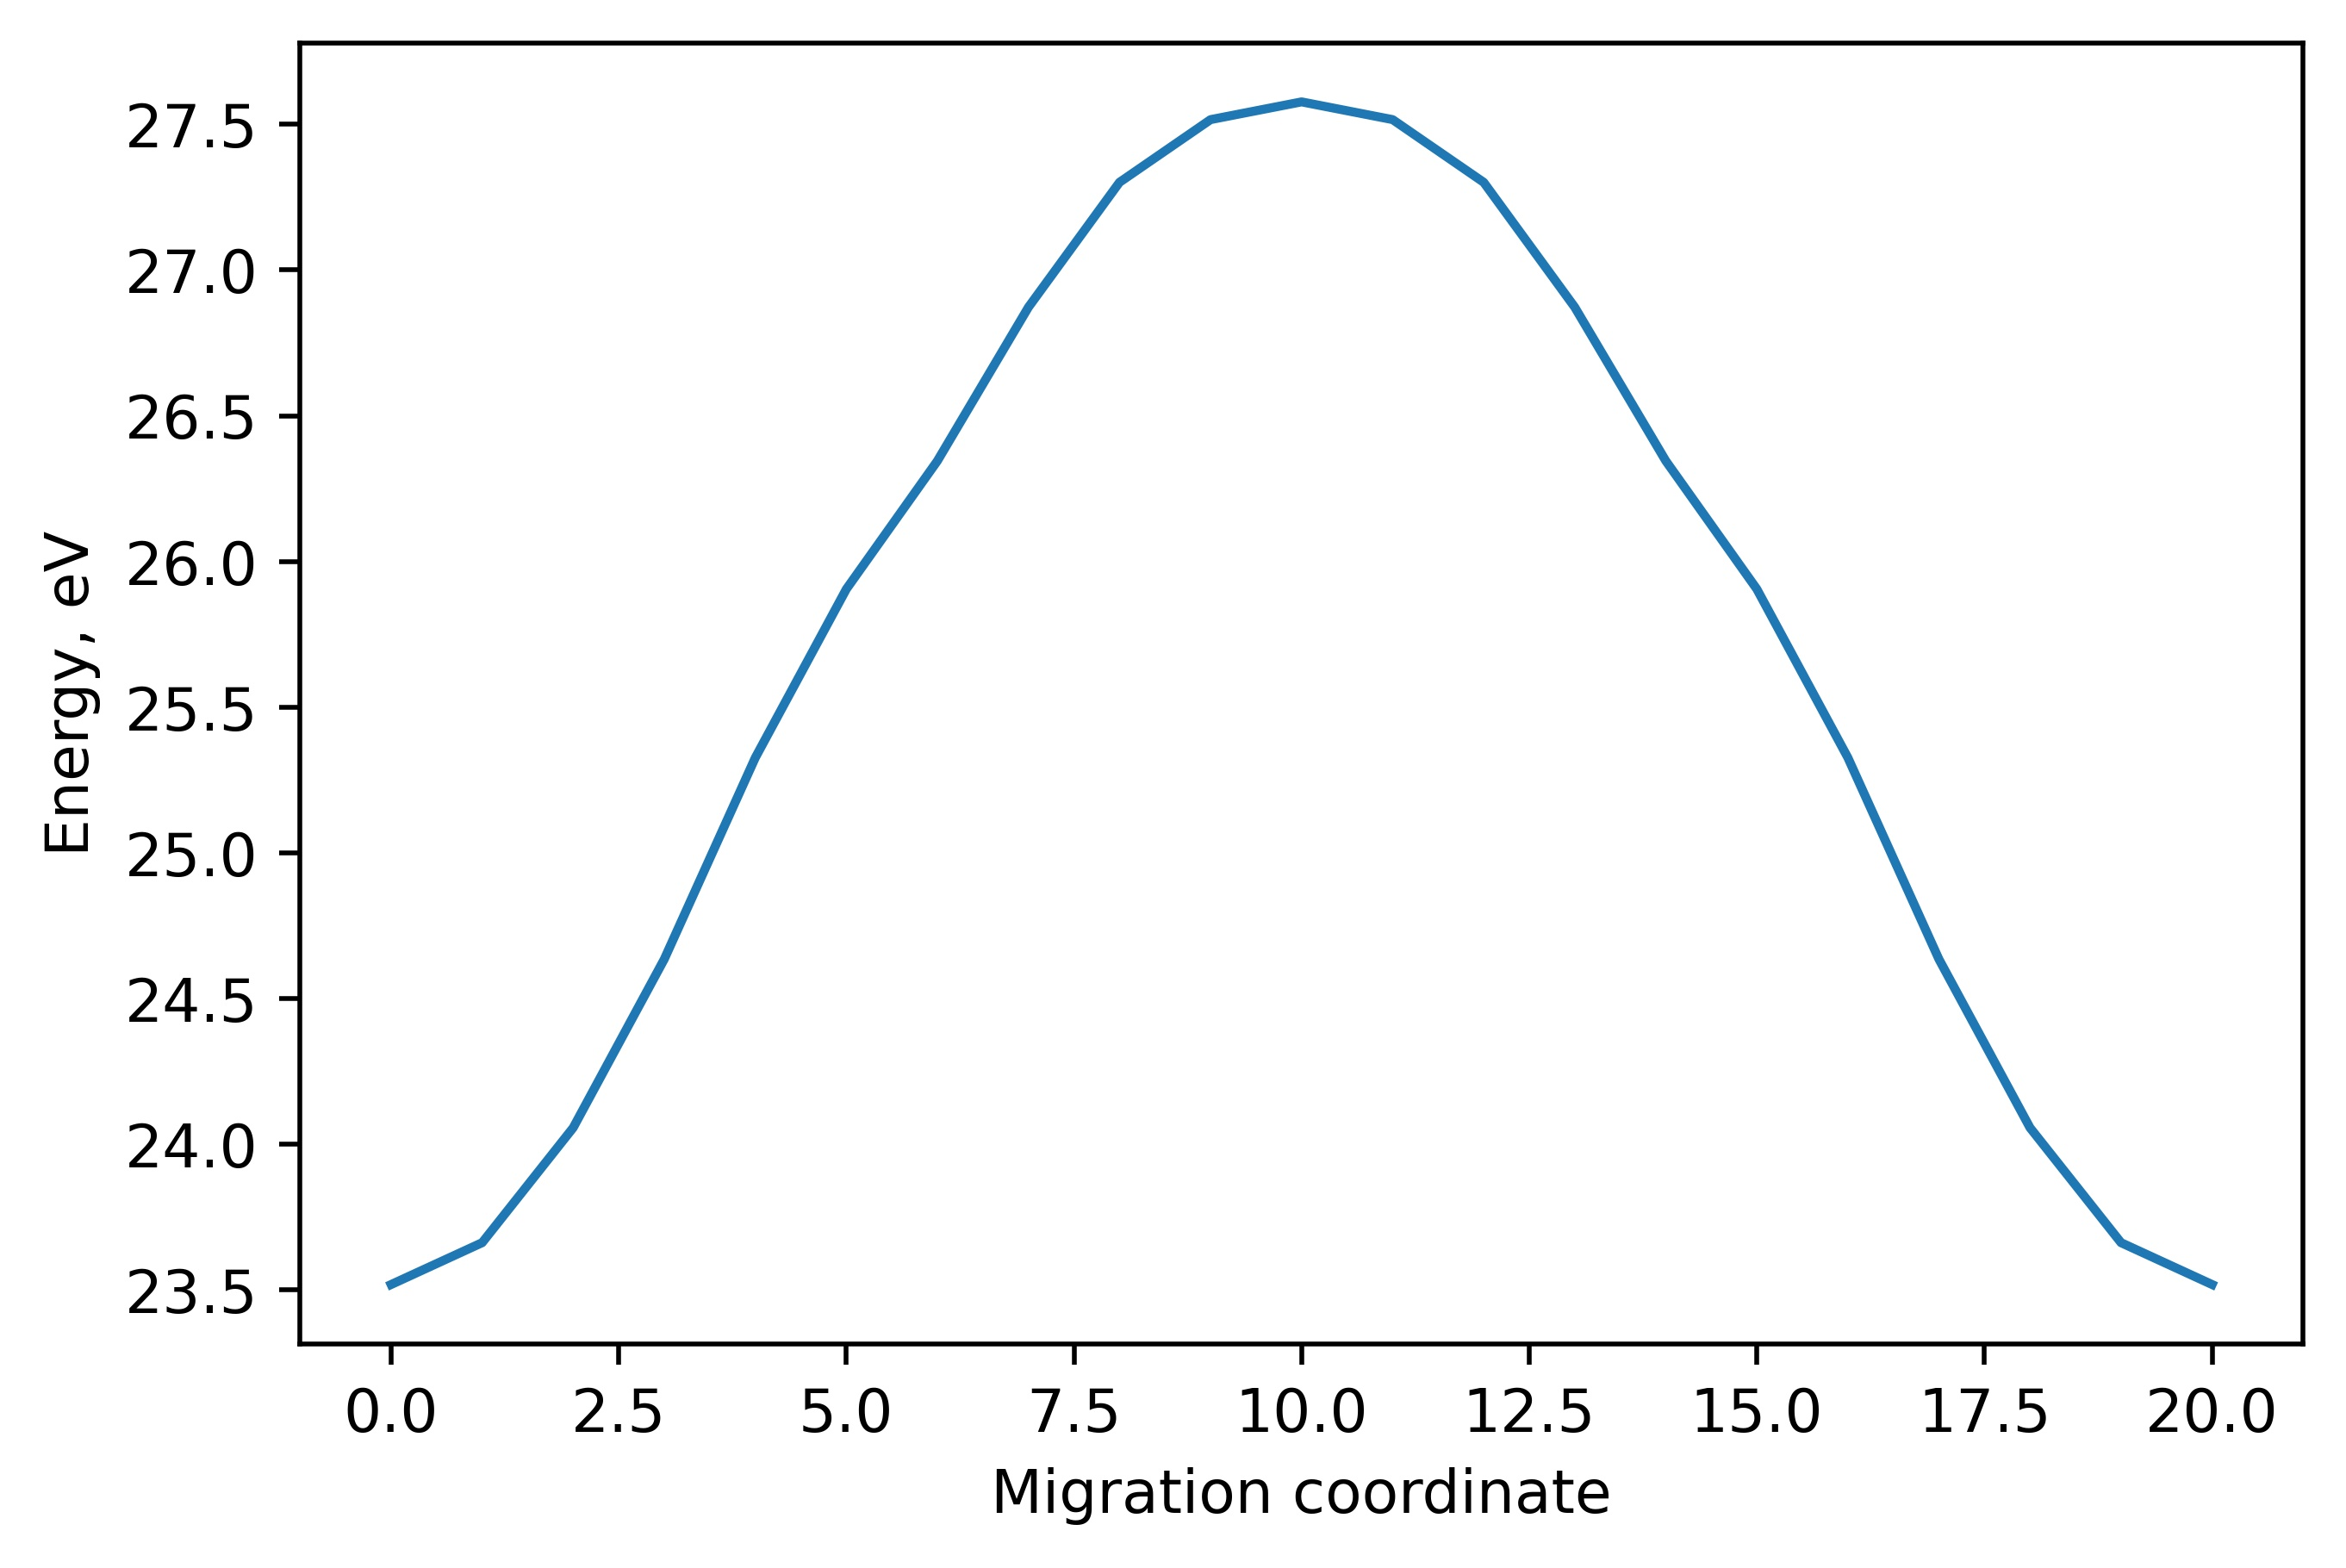
\includegraphics[width=10cm]{li3ocl_o_mig.jpg}
\caption{\label{li3ocl_o_mig.jpg} \ch{Li3OCl} oxide vacancy migration profile}
\end{figure}

\begin{figure}[h!]
\centering
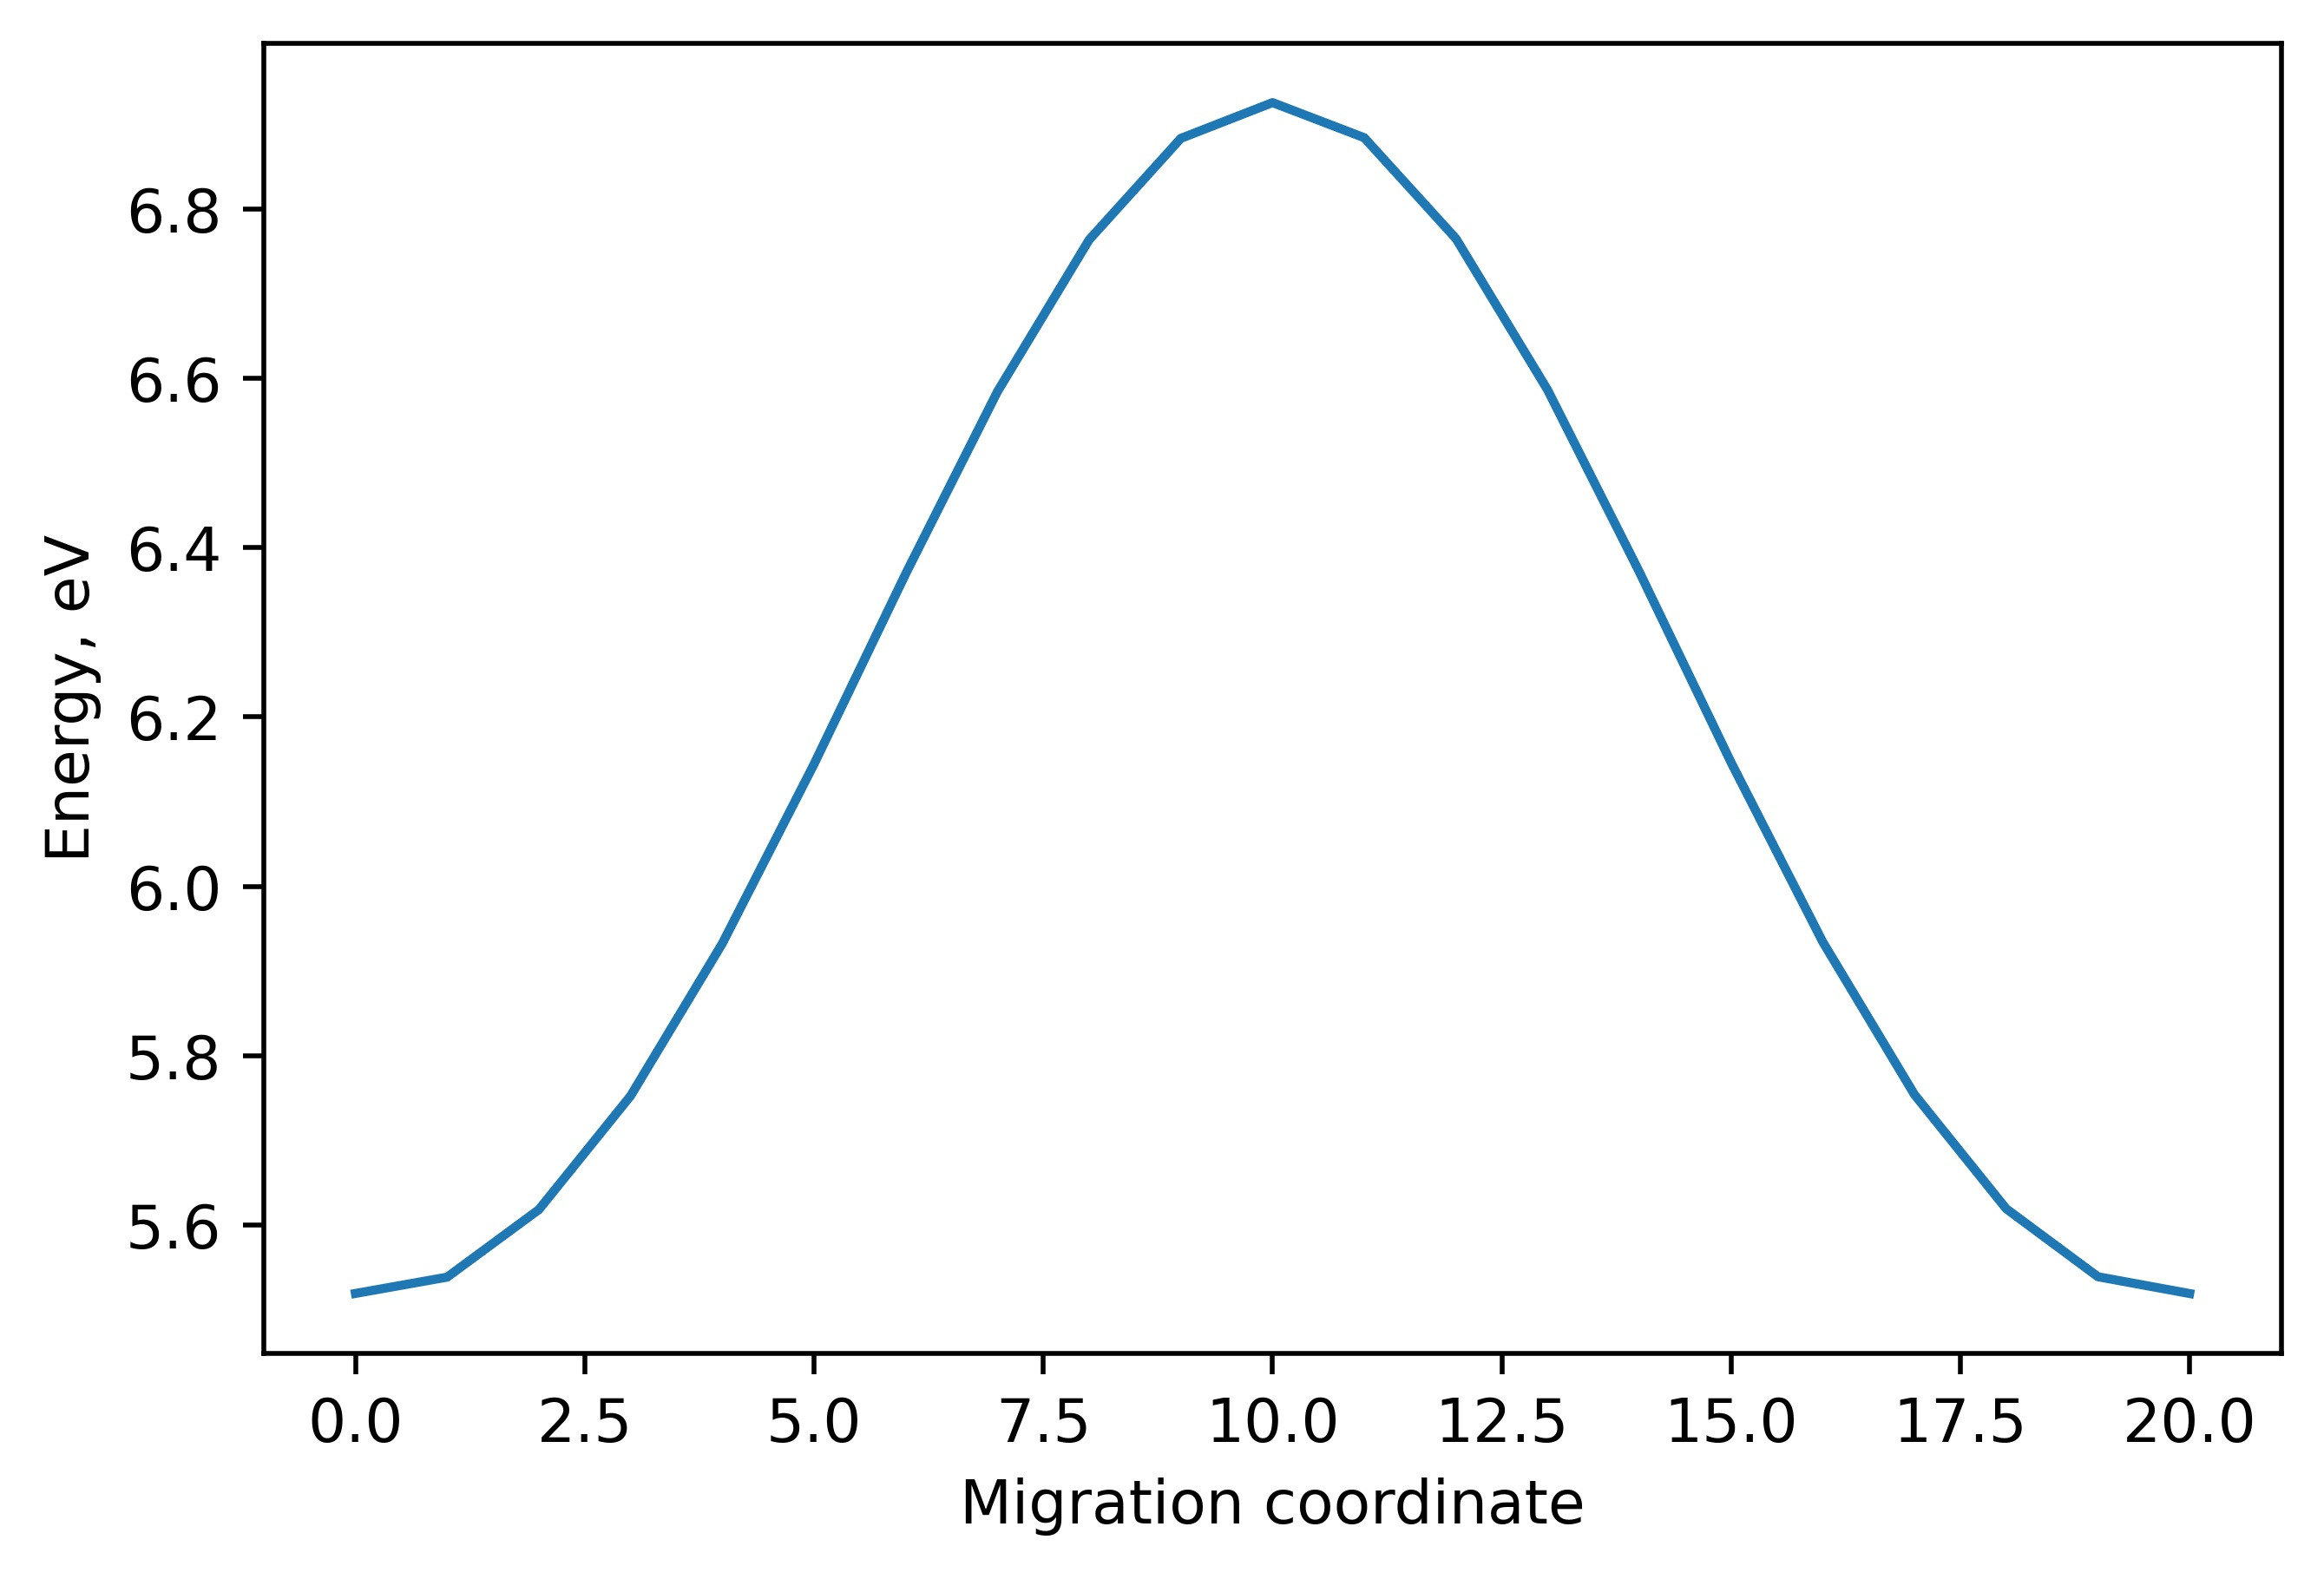
\includegraphics[width=10cm]{li3ocl_cl_mig.jpg}
\caption{\label{li3ocl_cl_mig.jpg} \ch{Li3OCl} chloride vacancy migration profile}
\end{figure}

\clearpage

\section{\ch{Na3OCl} data}

\begin{figure}[h]
\centering
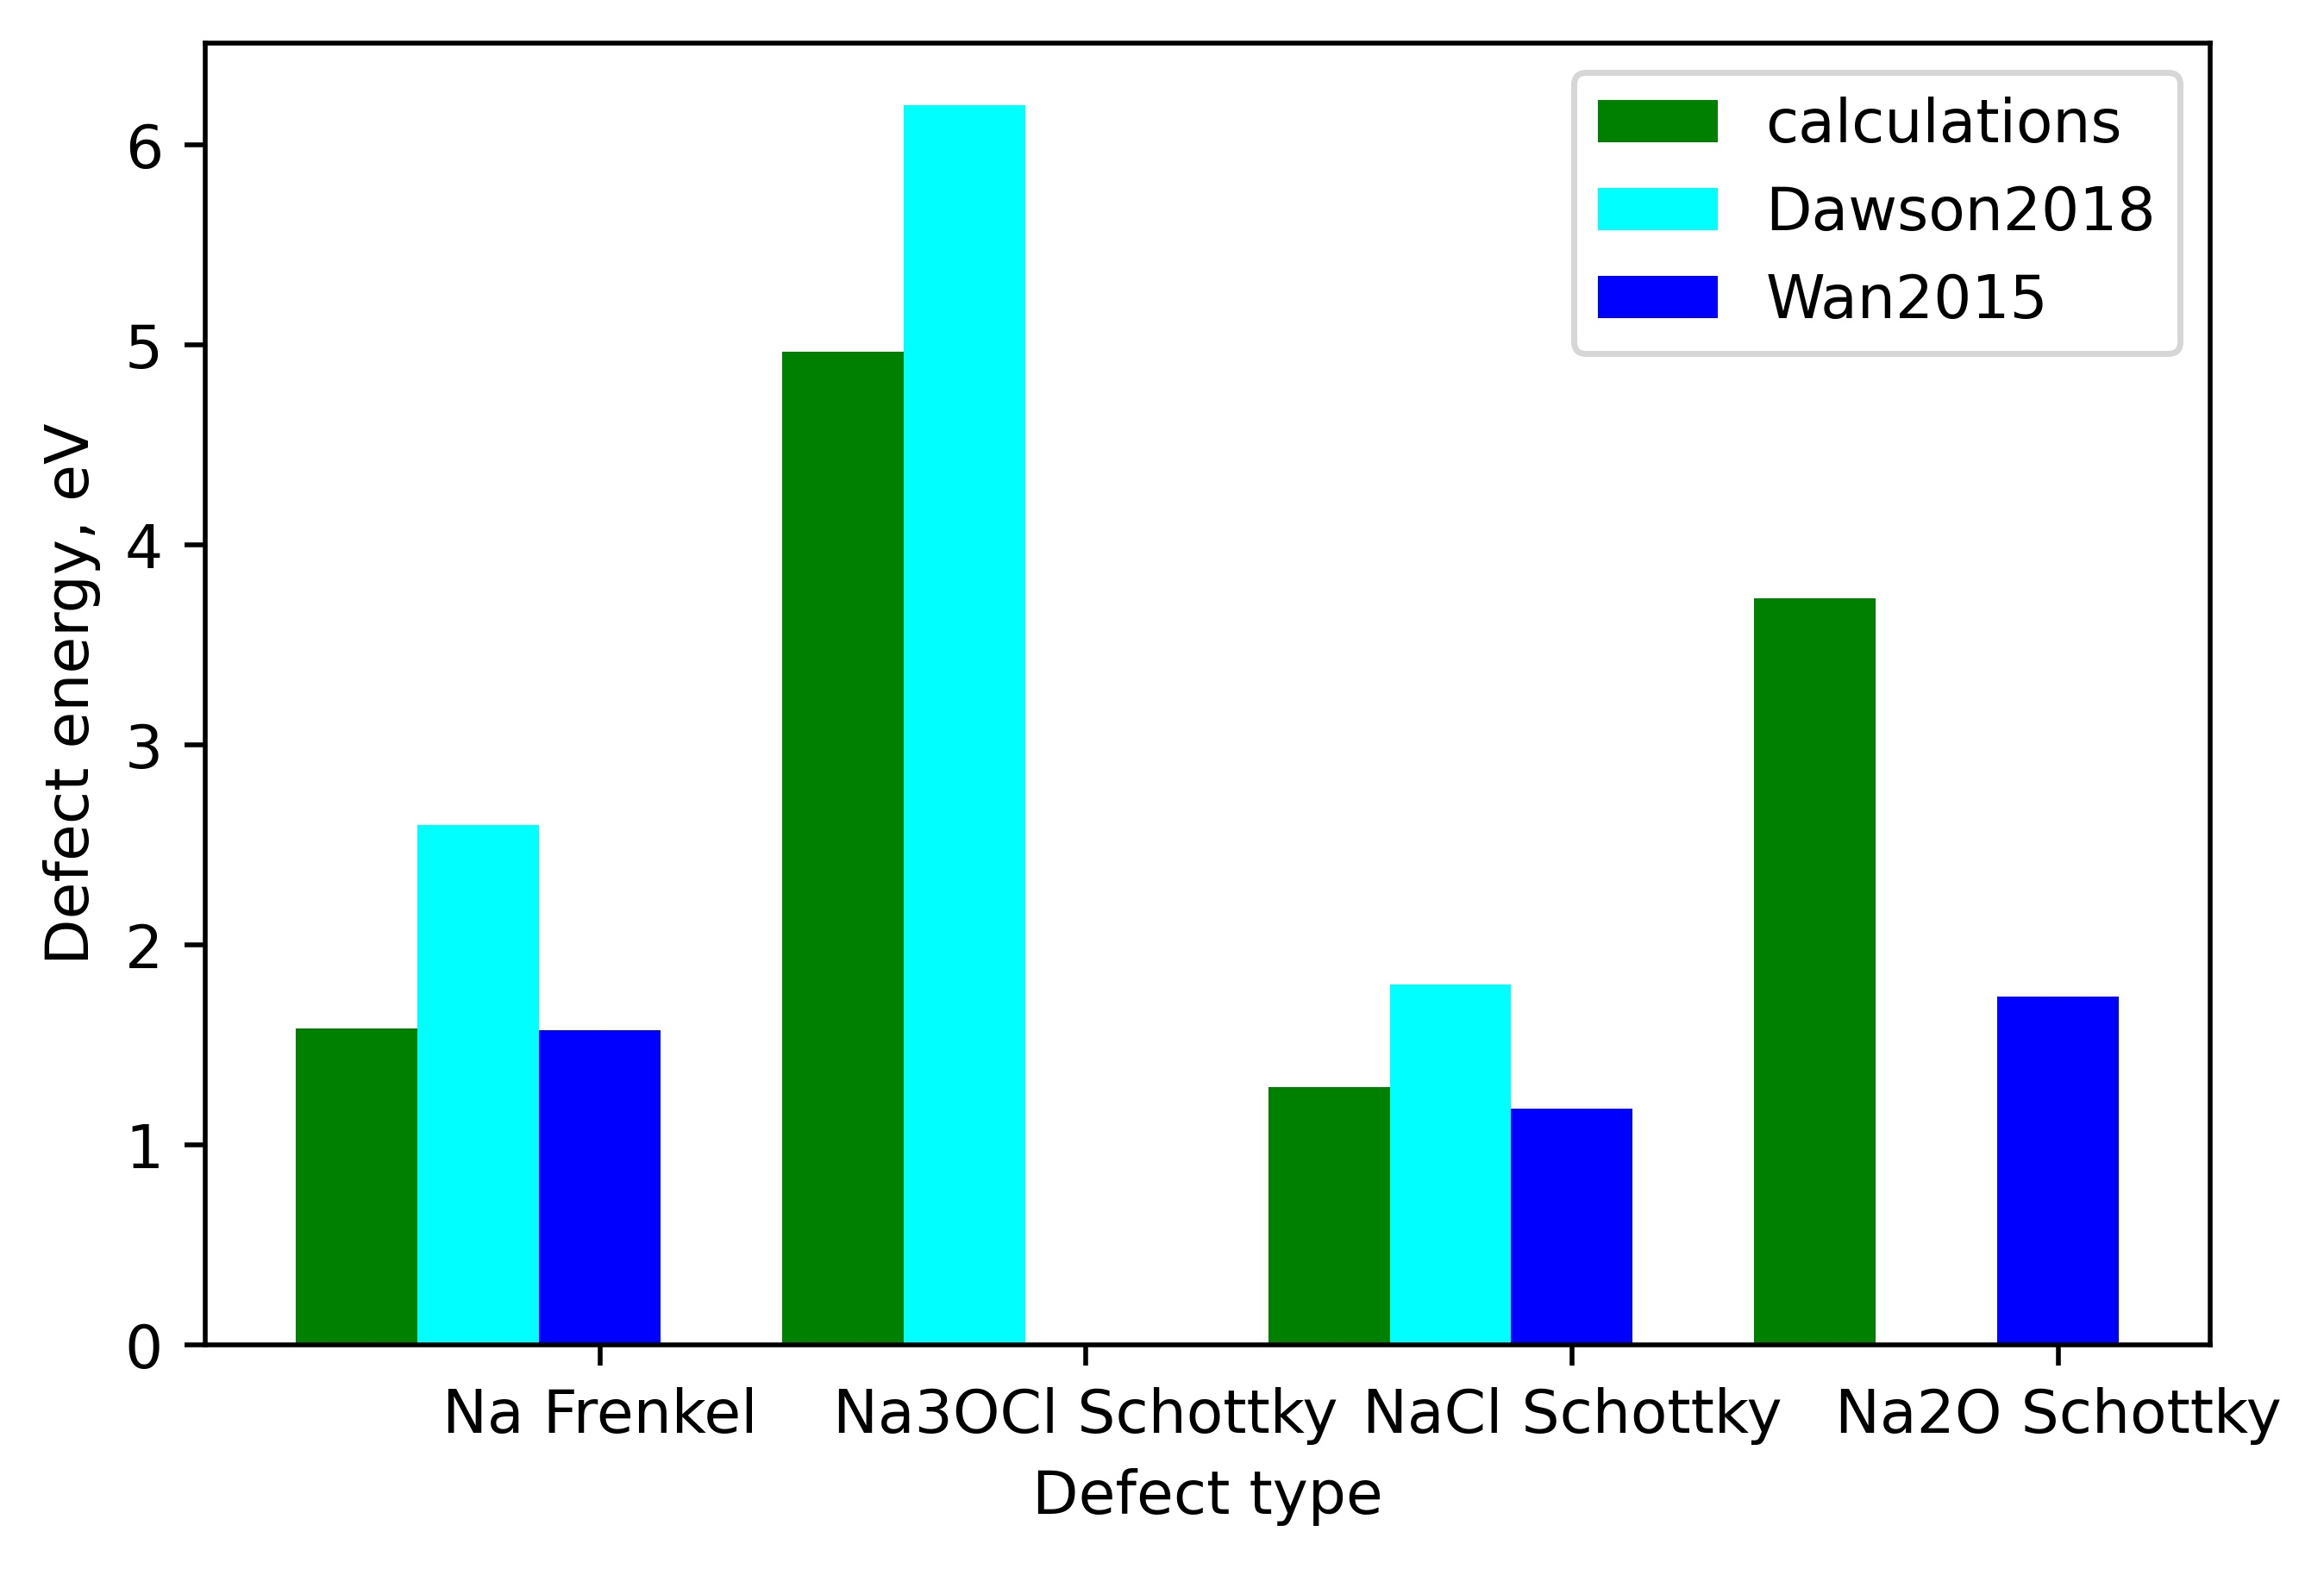
\includegraphics[width=10cm]{na3ocl_defects.jpg}
\caption{\label{na3ocl_doping.jpg} \ch{Na3OCl} defects}
\end{figure}

\begin{figure}[h]
\centering
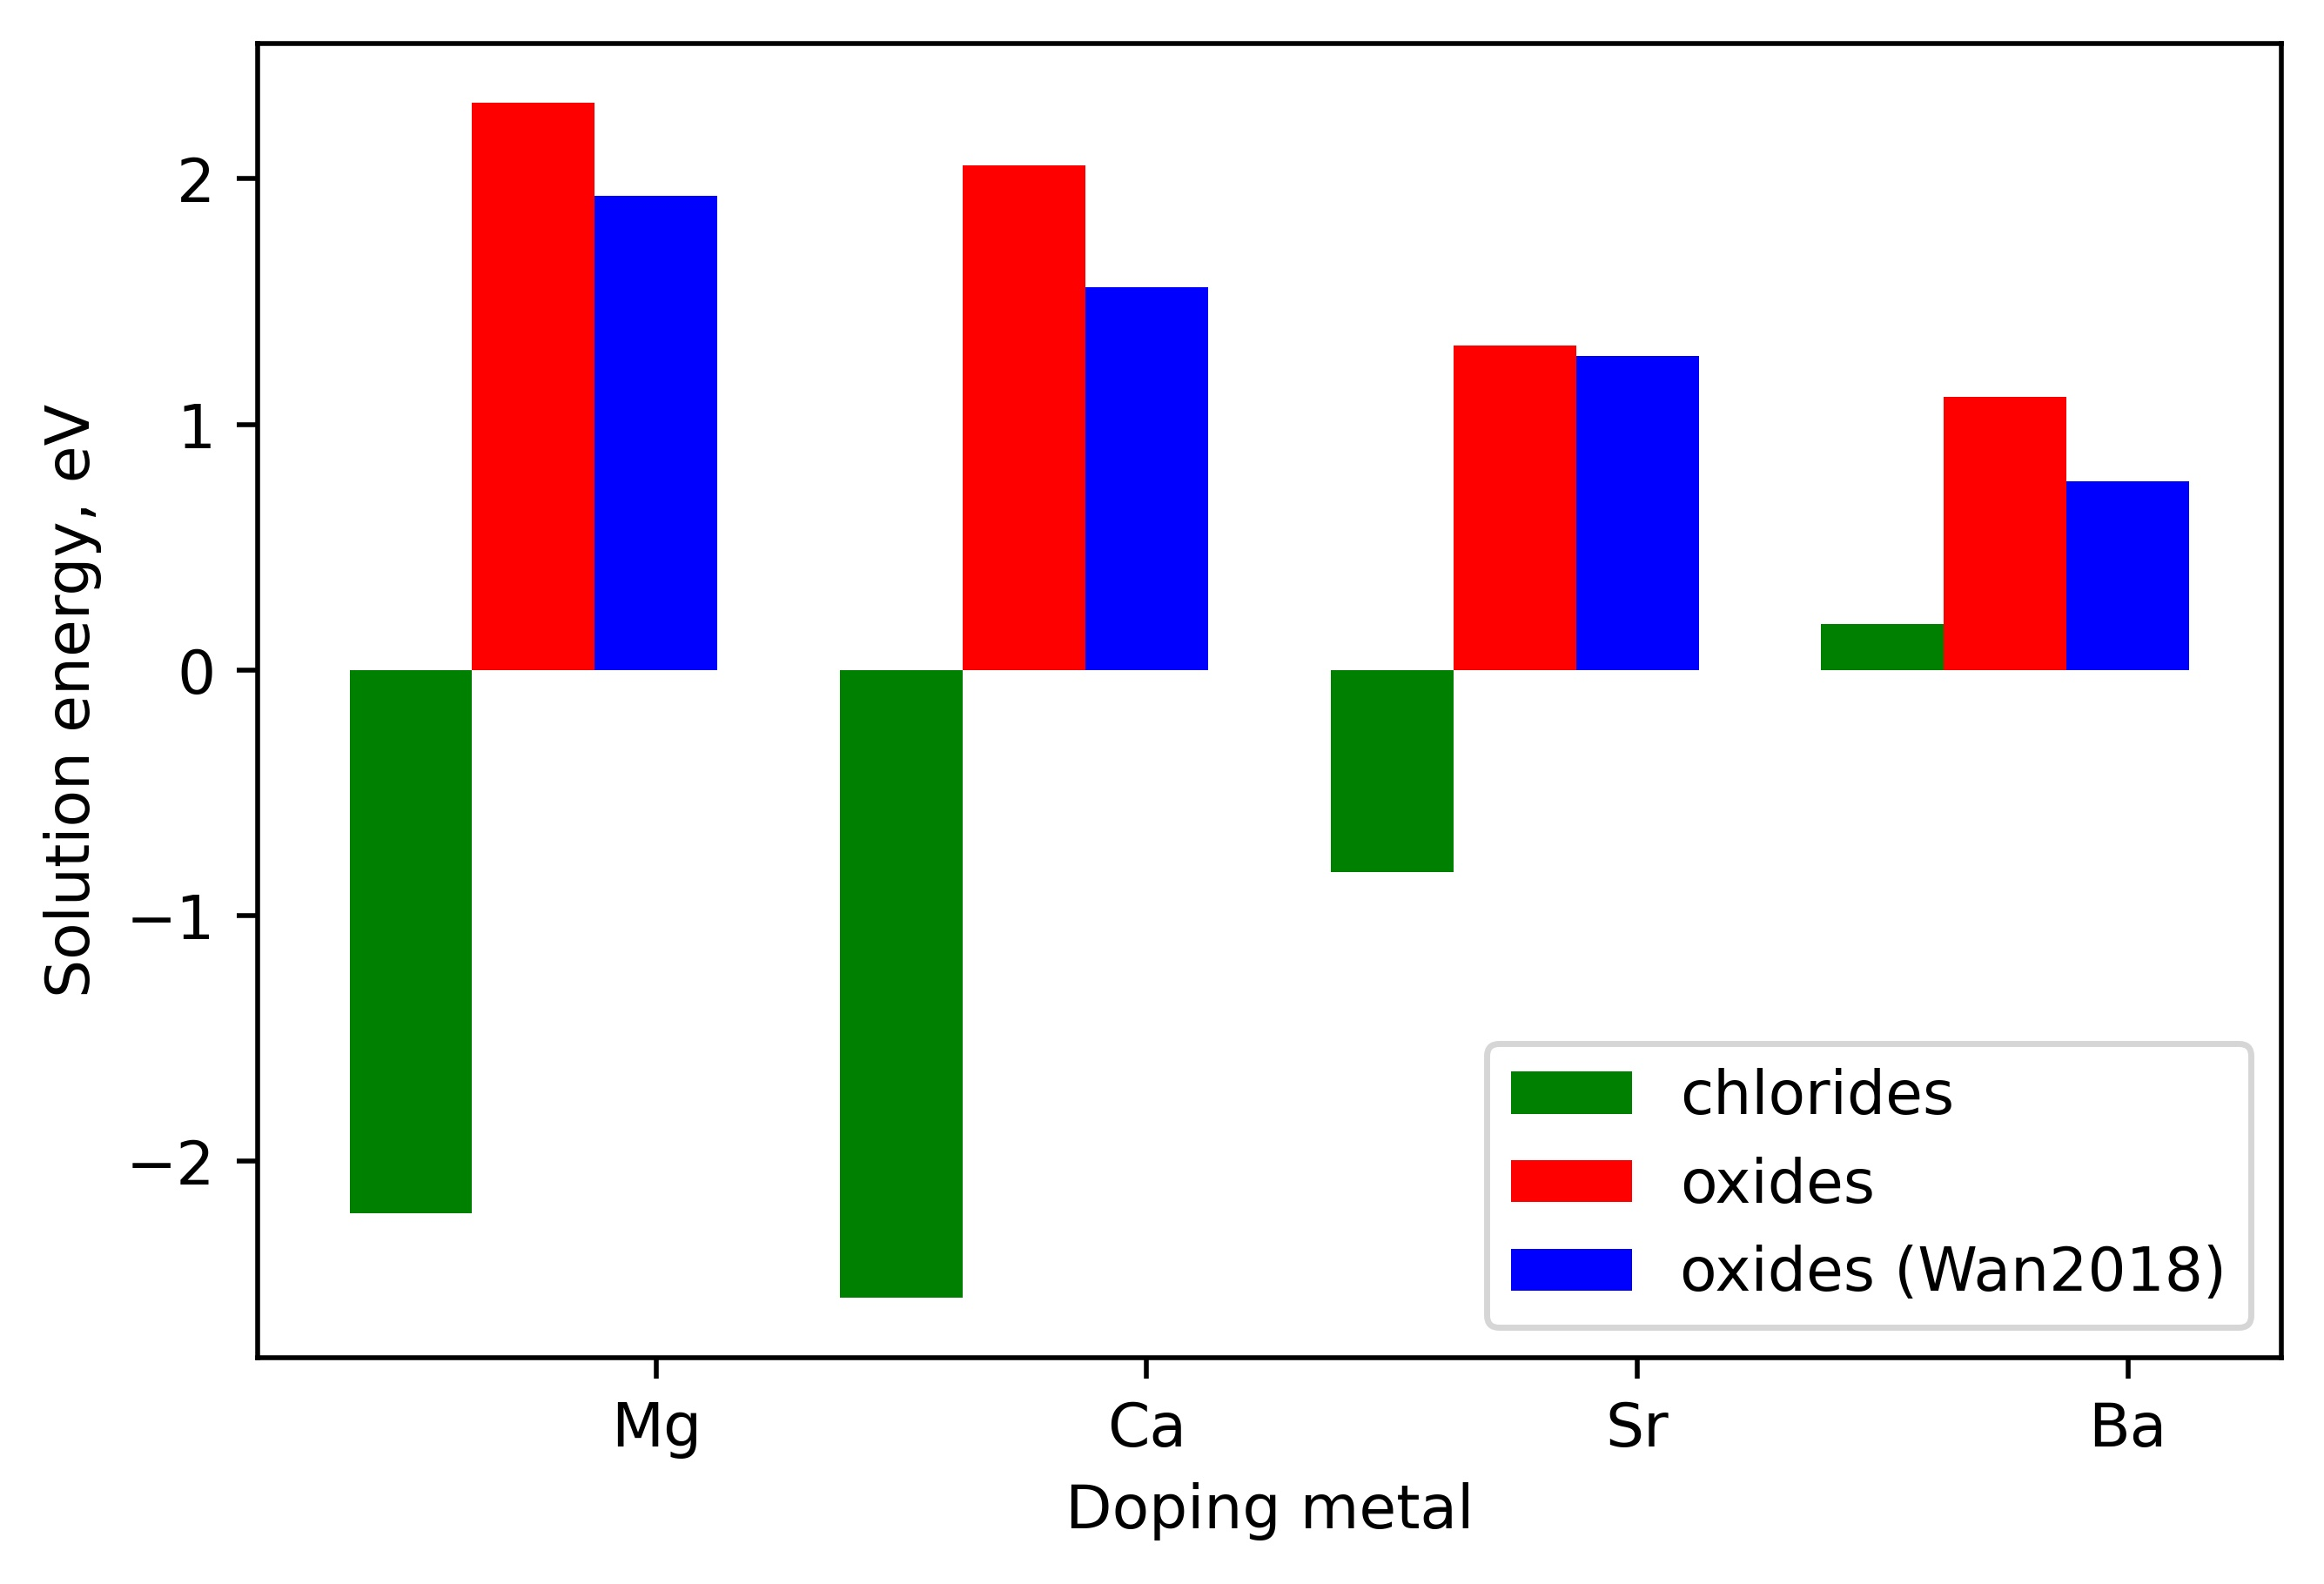
\includegraphics[width=10cm]{na3ocl_doping.jpg}
\caption{\label{na3ocl_doping.jpg} \ch{Na3OCl} doping}
\end{figure}

\begin{figure}[h]
\centering
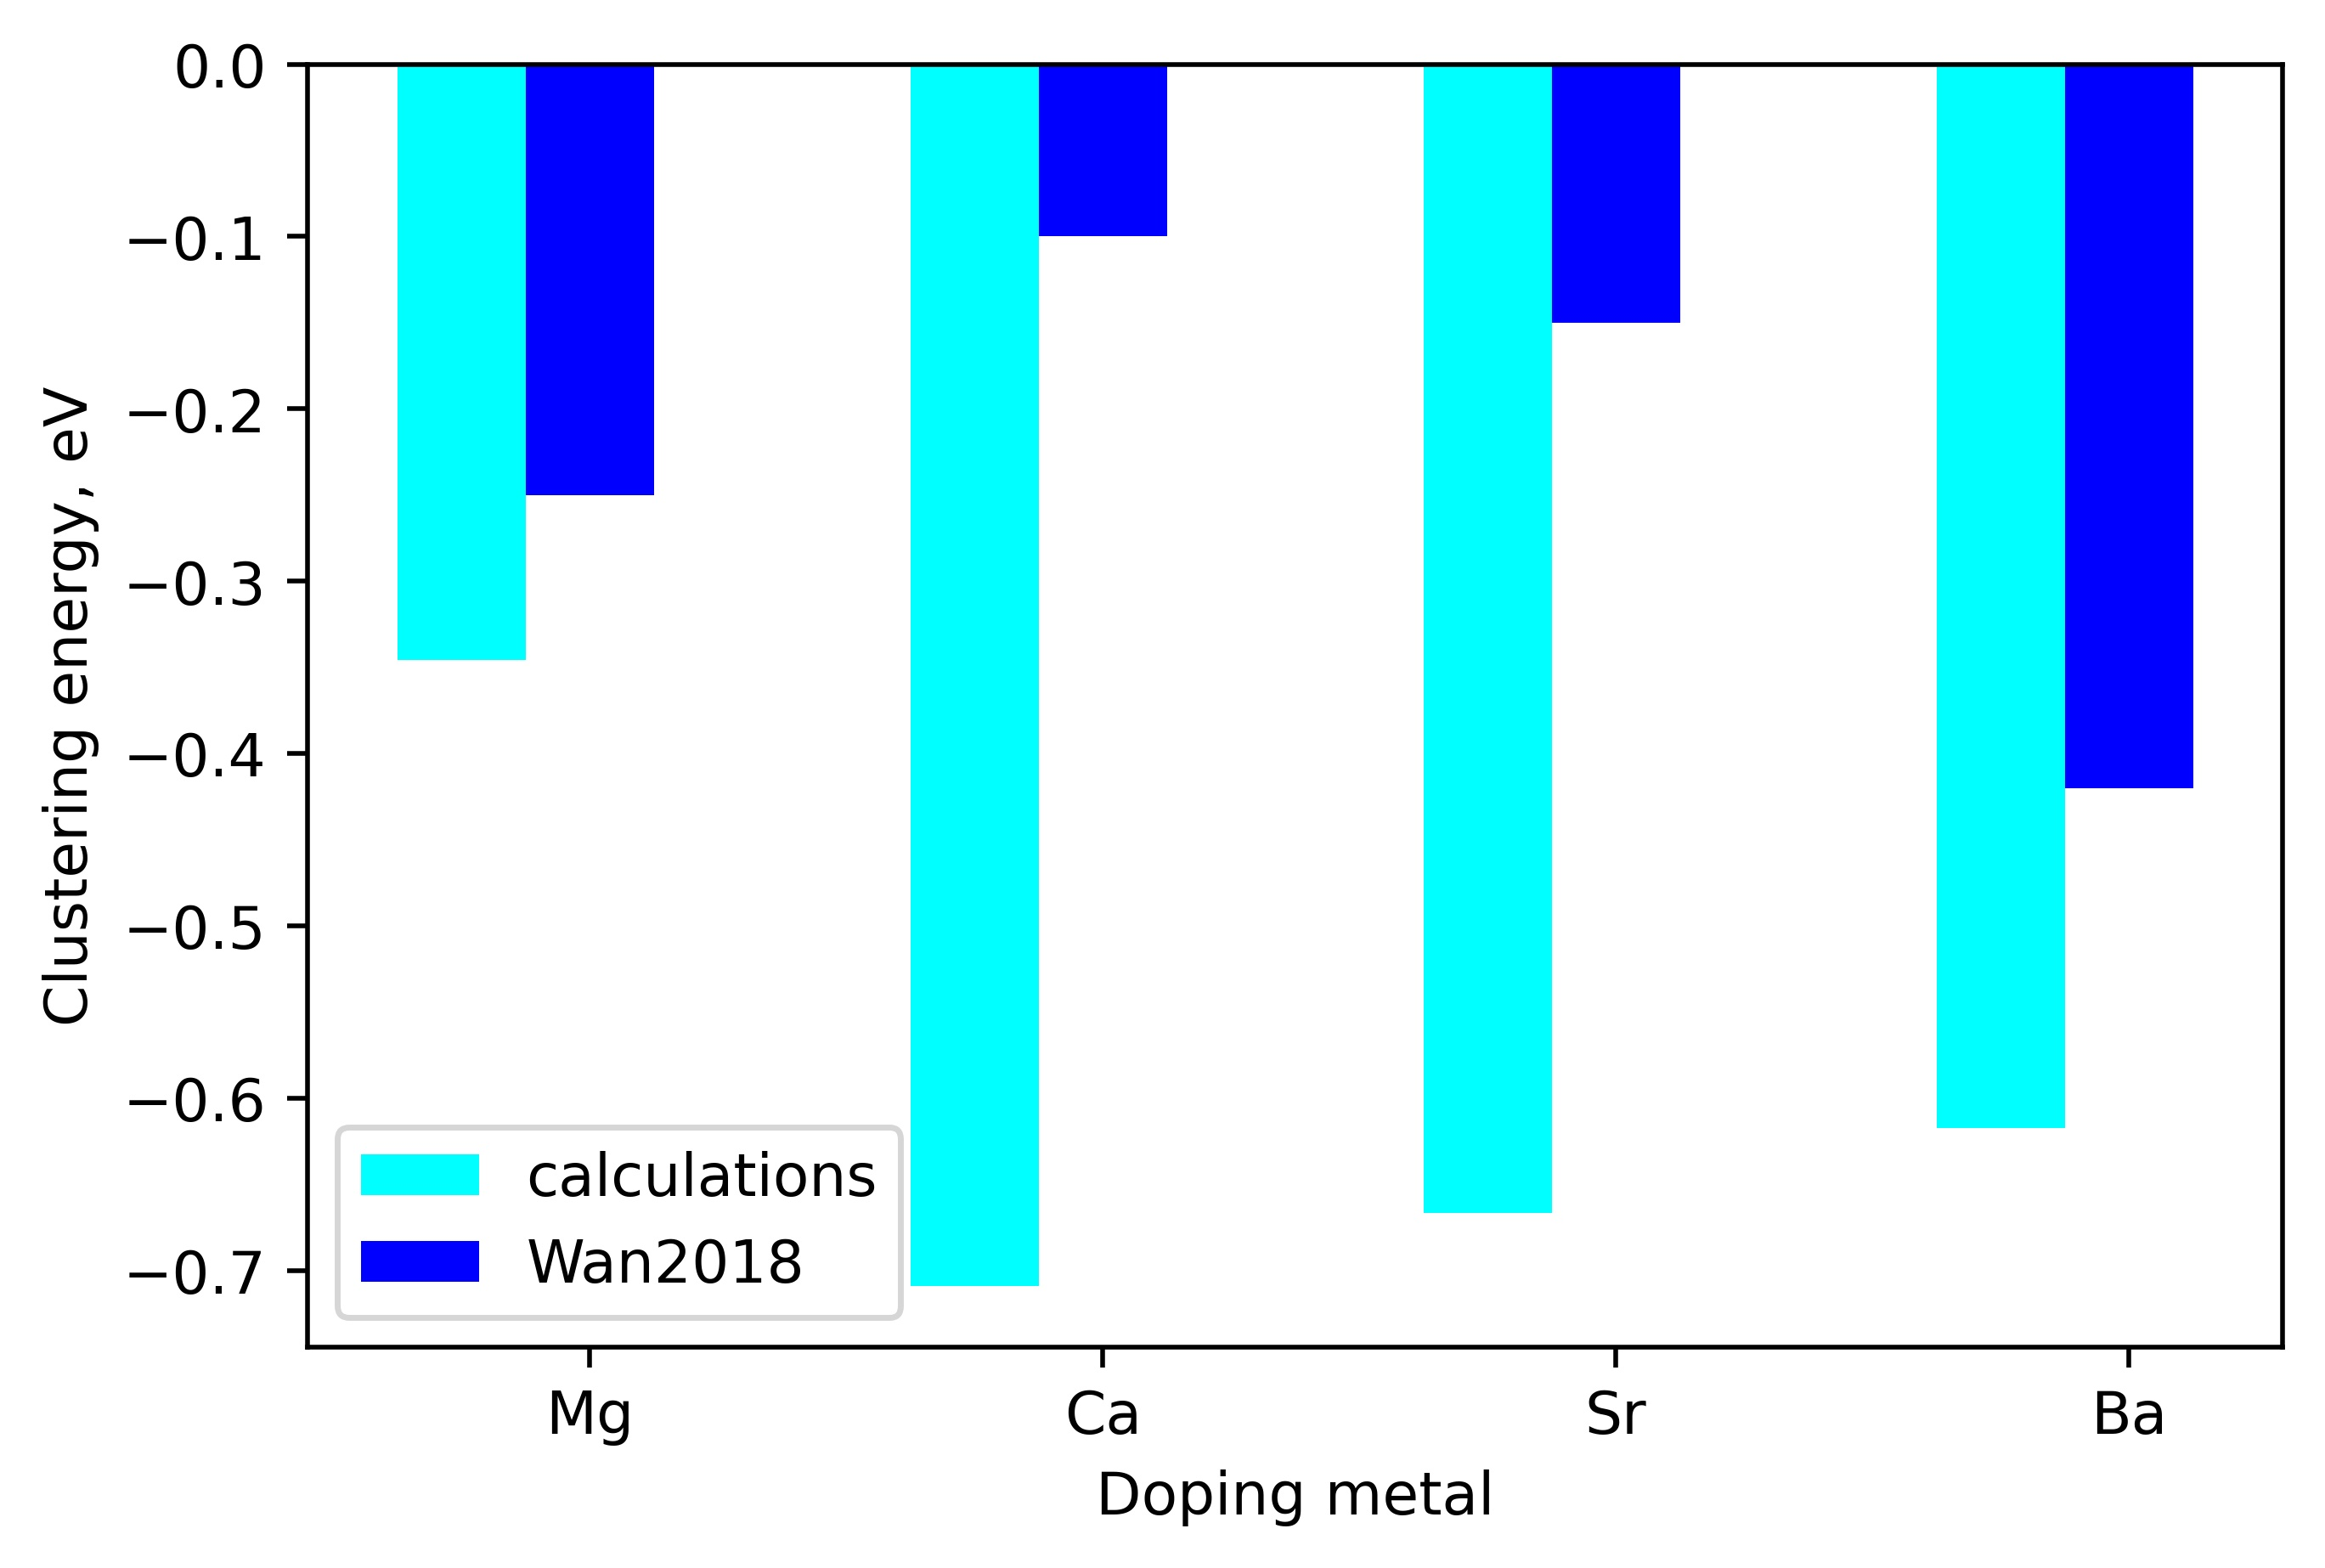
\includegraphics[width=10cm]{na3ocl_clustering.jpg}
\caption{\label{na3ocl_clustering.jpg} \ch{Na3OCl} clustering}
\end{figure}

\begin{figure}[h]
\centering
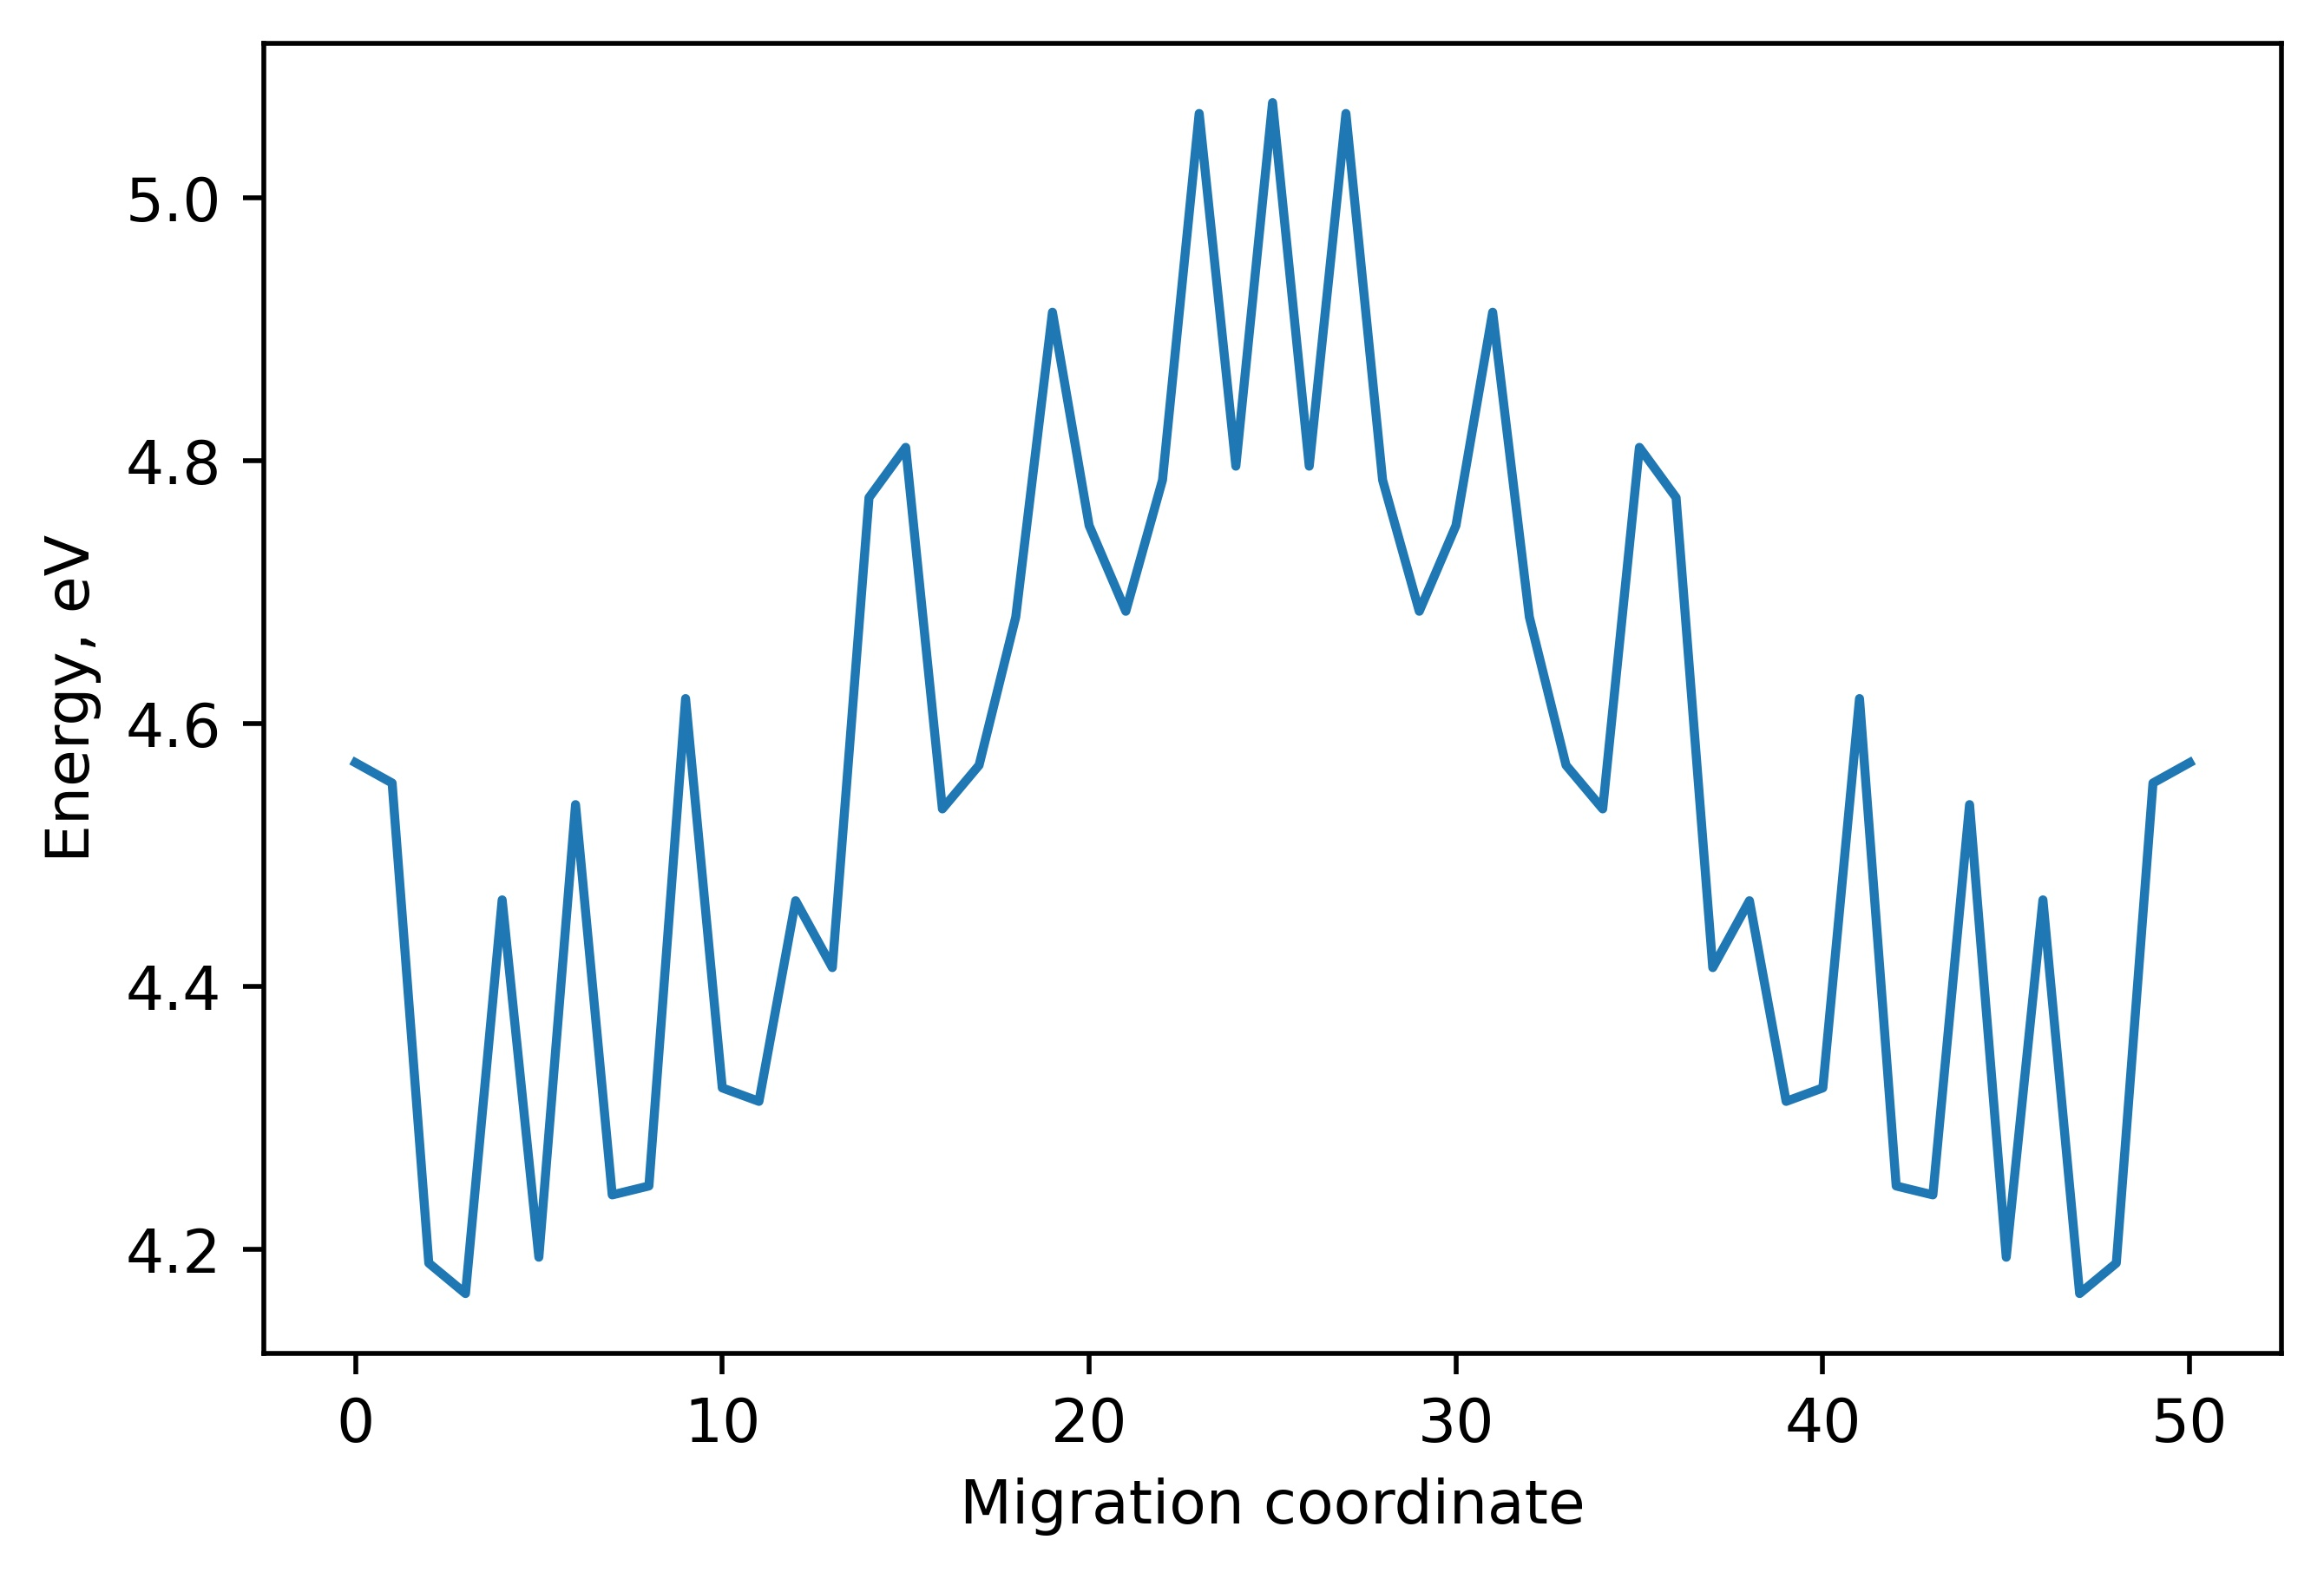
\includegraphics[width=10cm]{na3ocl_namig_fix.jpg}
\caption{\label{na3ocl_namig_fix.jpg} Na migration in \ch{Na3OCl} with migration coordinate along line from (0.5 0.5 0) to (0.5 0 0.5) fixed in all dimensions}
\end{figure}

\begin{figure}[h]
\centering
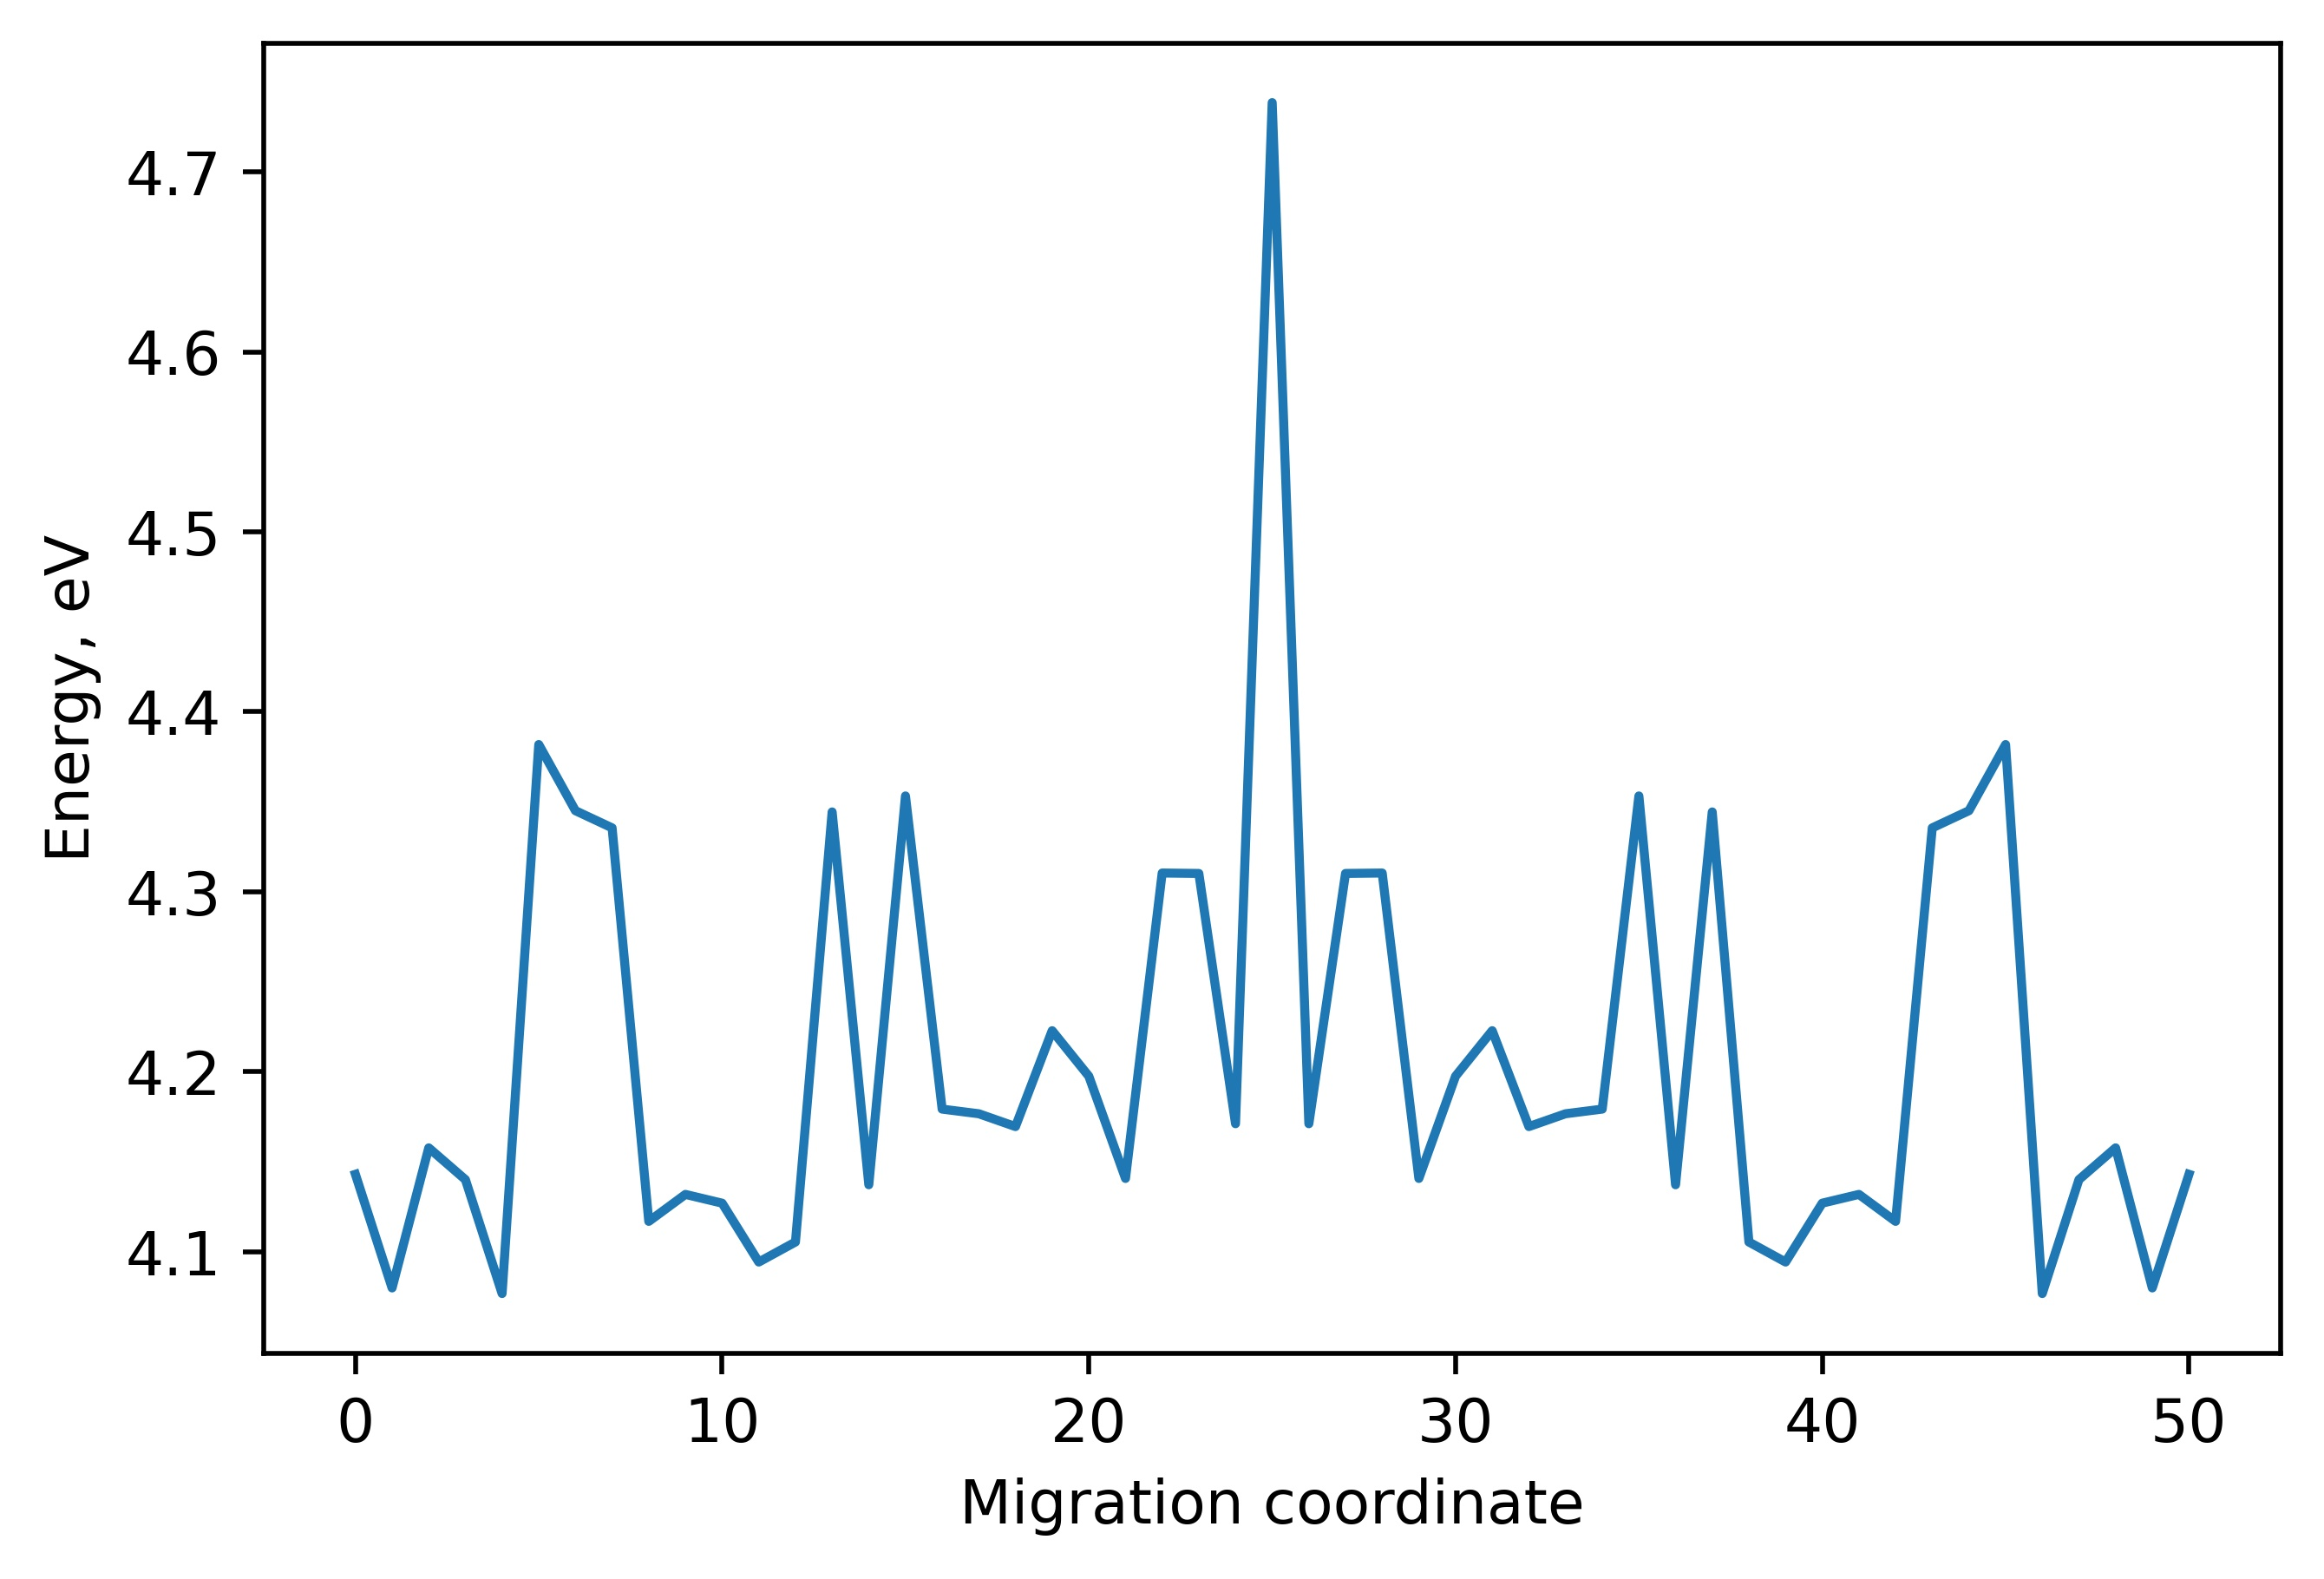
\includegraphics[width=10cm]{na3ocl_namig_fixx.jpg}
\caption{\label{na3ocl_namig_fixx.jpg} Na migration in \ch{Na3OCl} with migration coordinate along line from (0.5 0.5 0) to (0.5 0 0.5) fixed in the $x$ dimension}
\end{figure}

\begin{figure}[h]
\centering
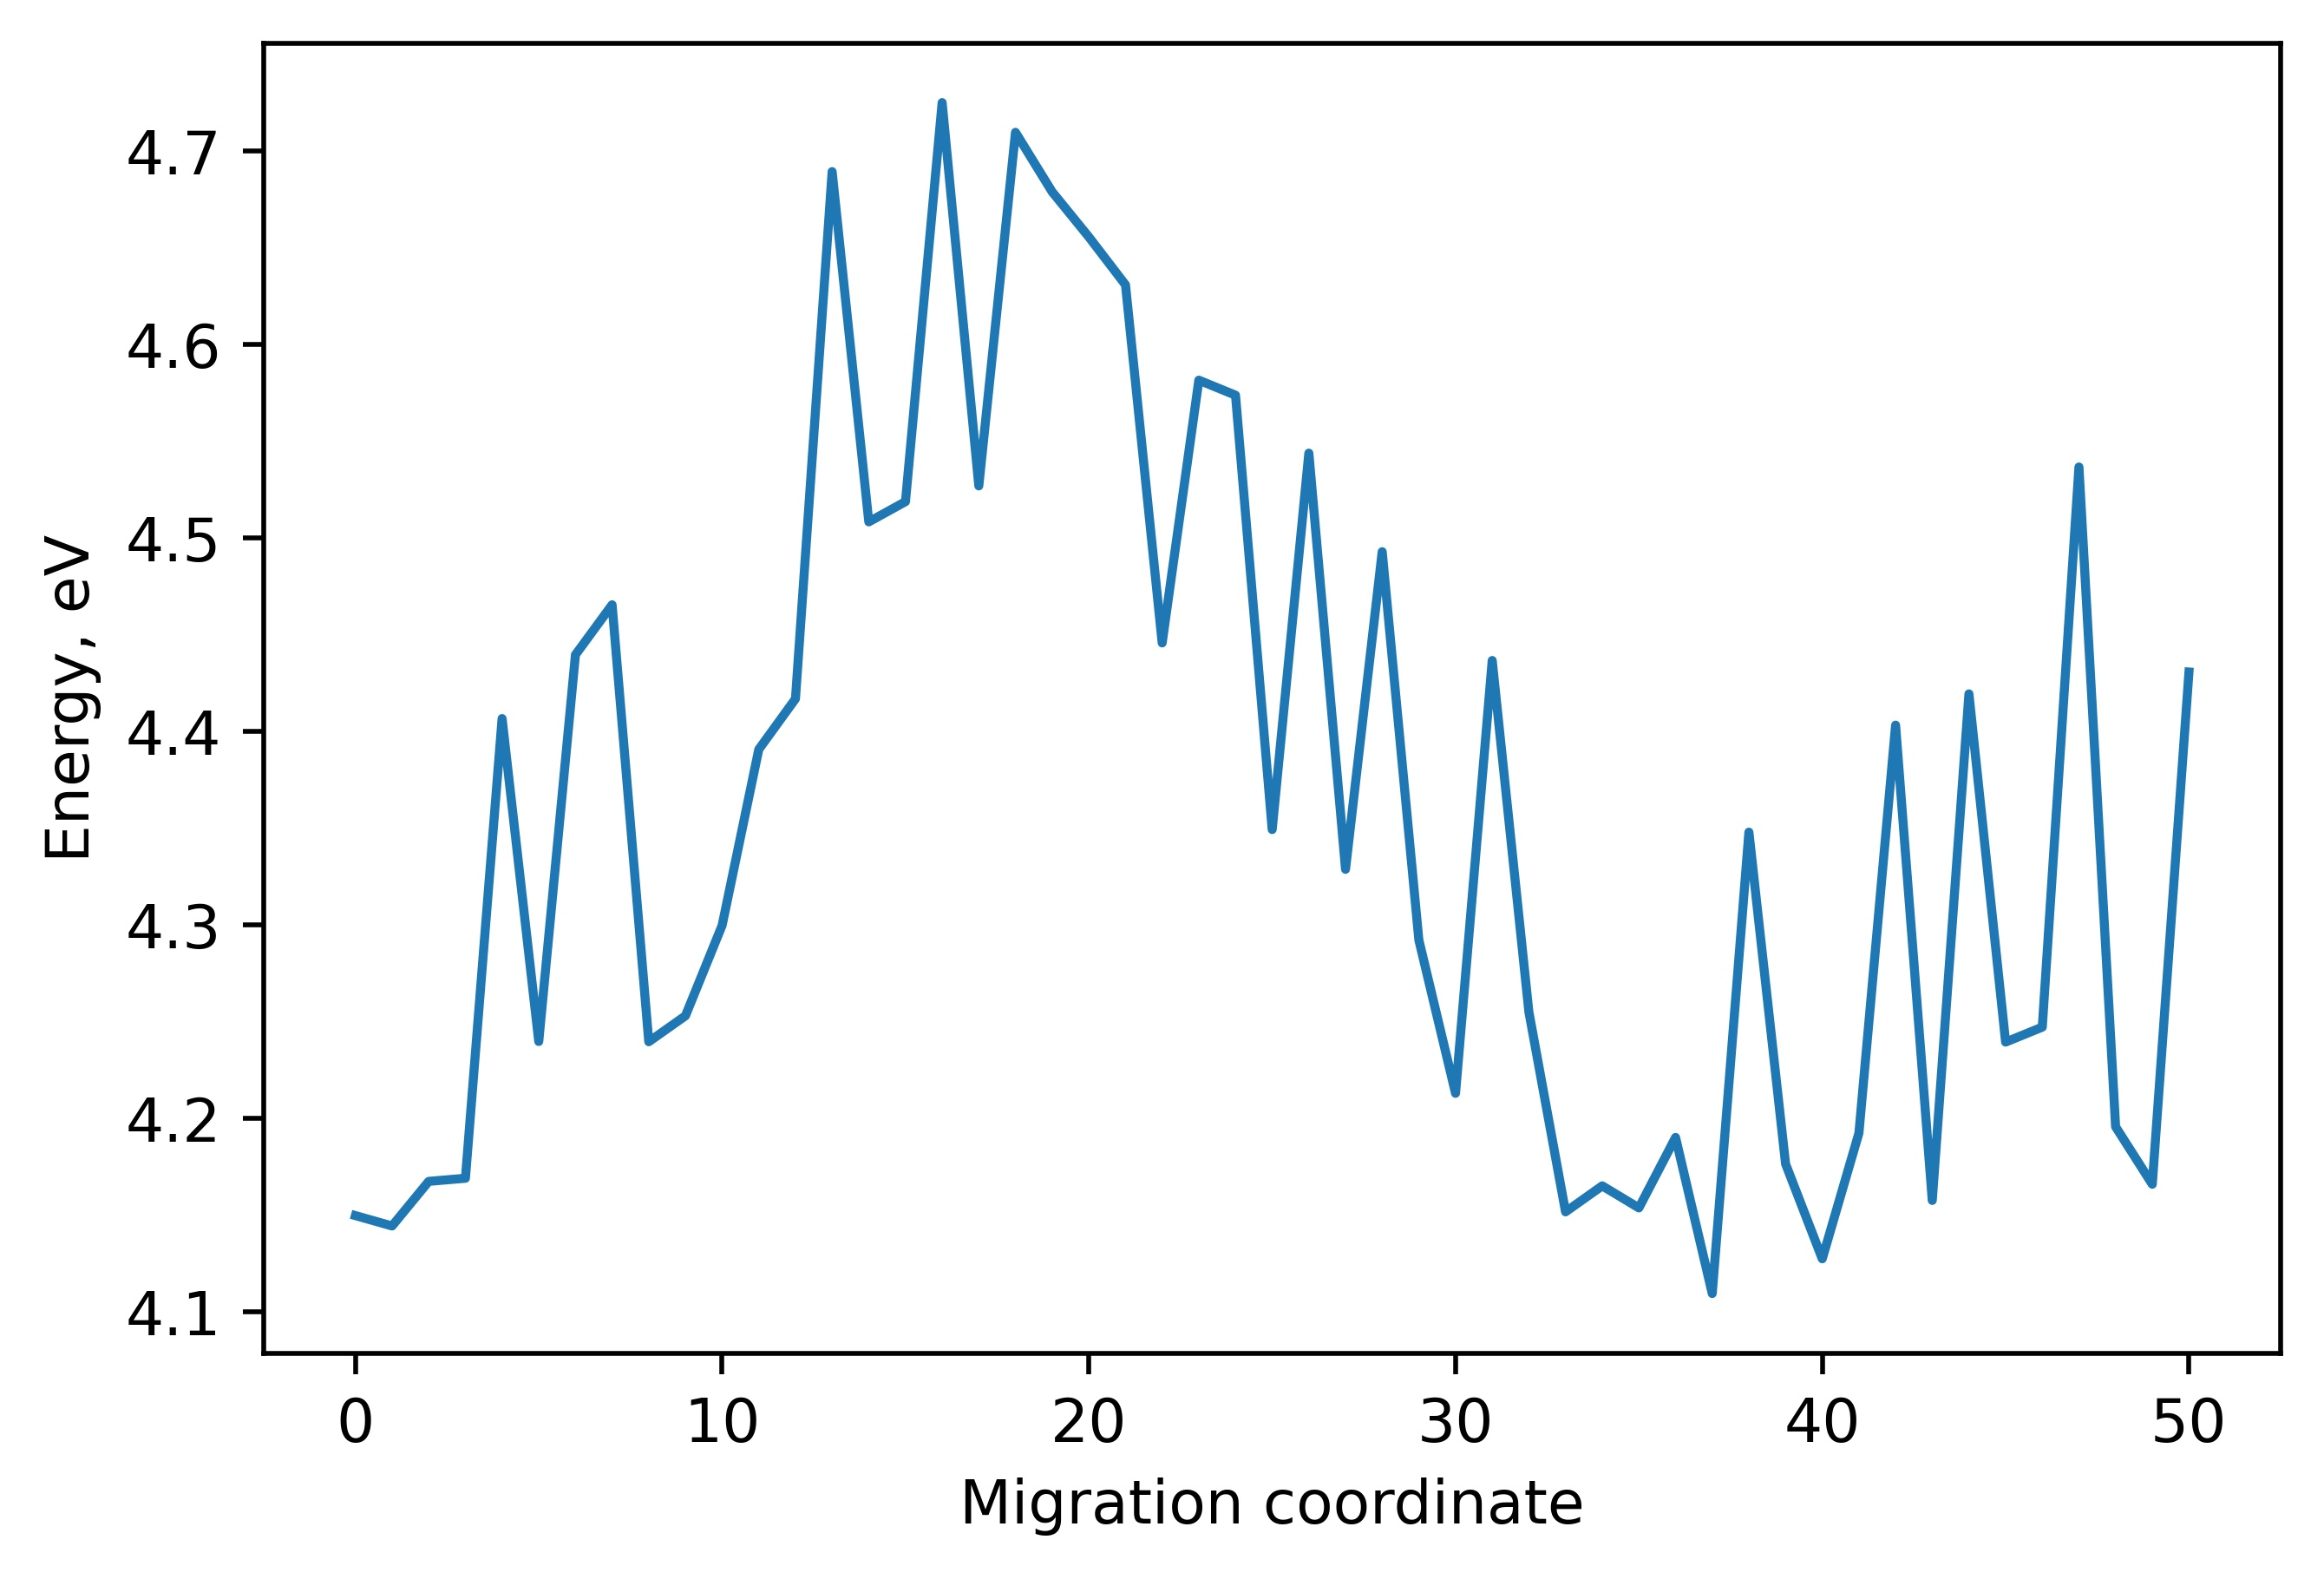
\includegraphics[width=10cm]{na3ocl_namig_fixy.jpg}
\caption{\label{na3ocl_namig_fixy.jpg} Na migration in \ch{Na3OCl} with migration coordinate along line from (0.5 0.5 0) to (0.5 0 0.5) fixed in the $y$ dimension}
\end{figure}

\begin{figure}[h]
\centering
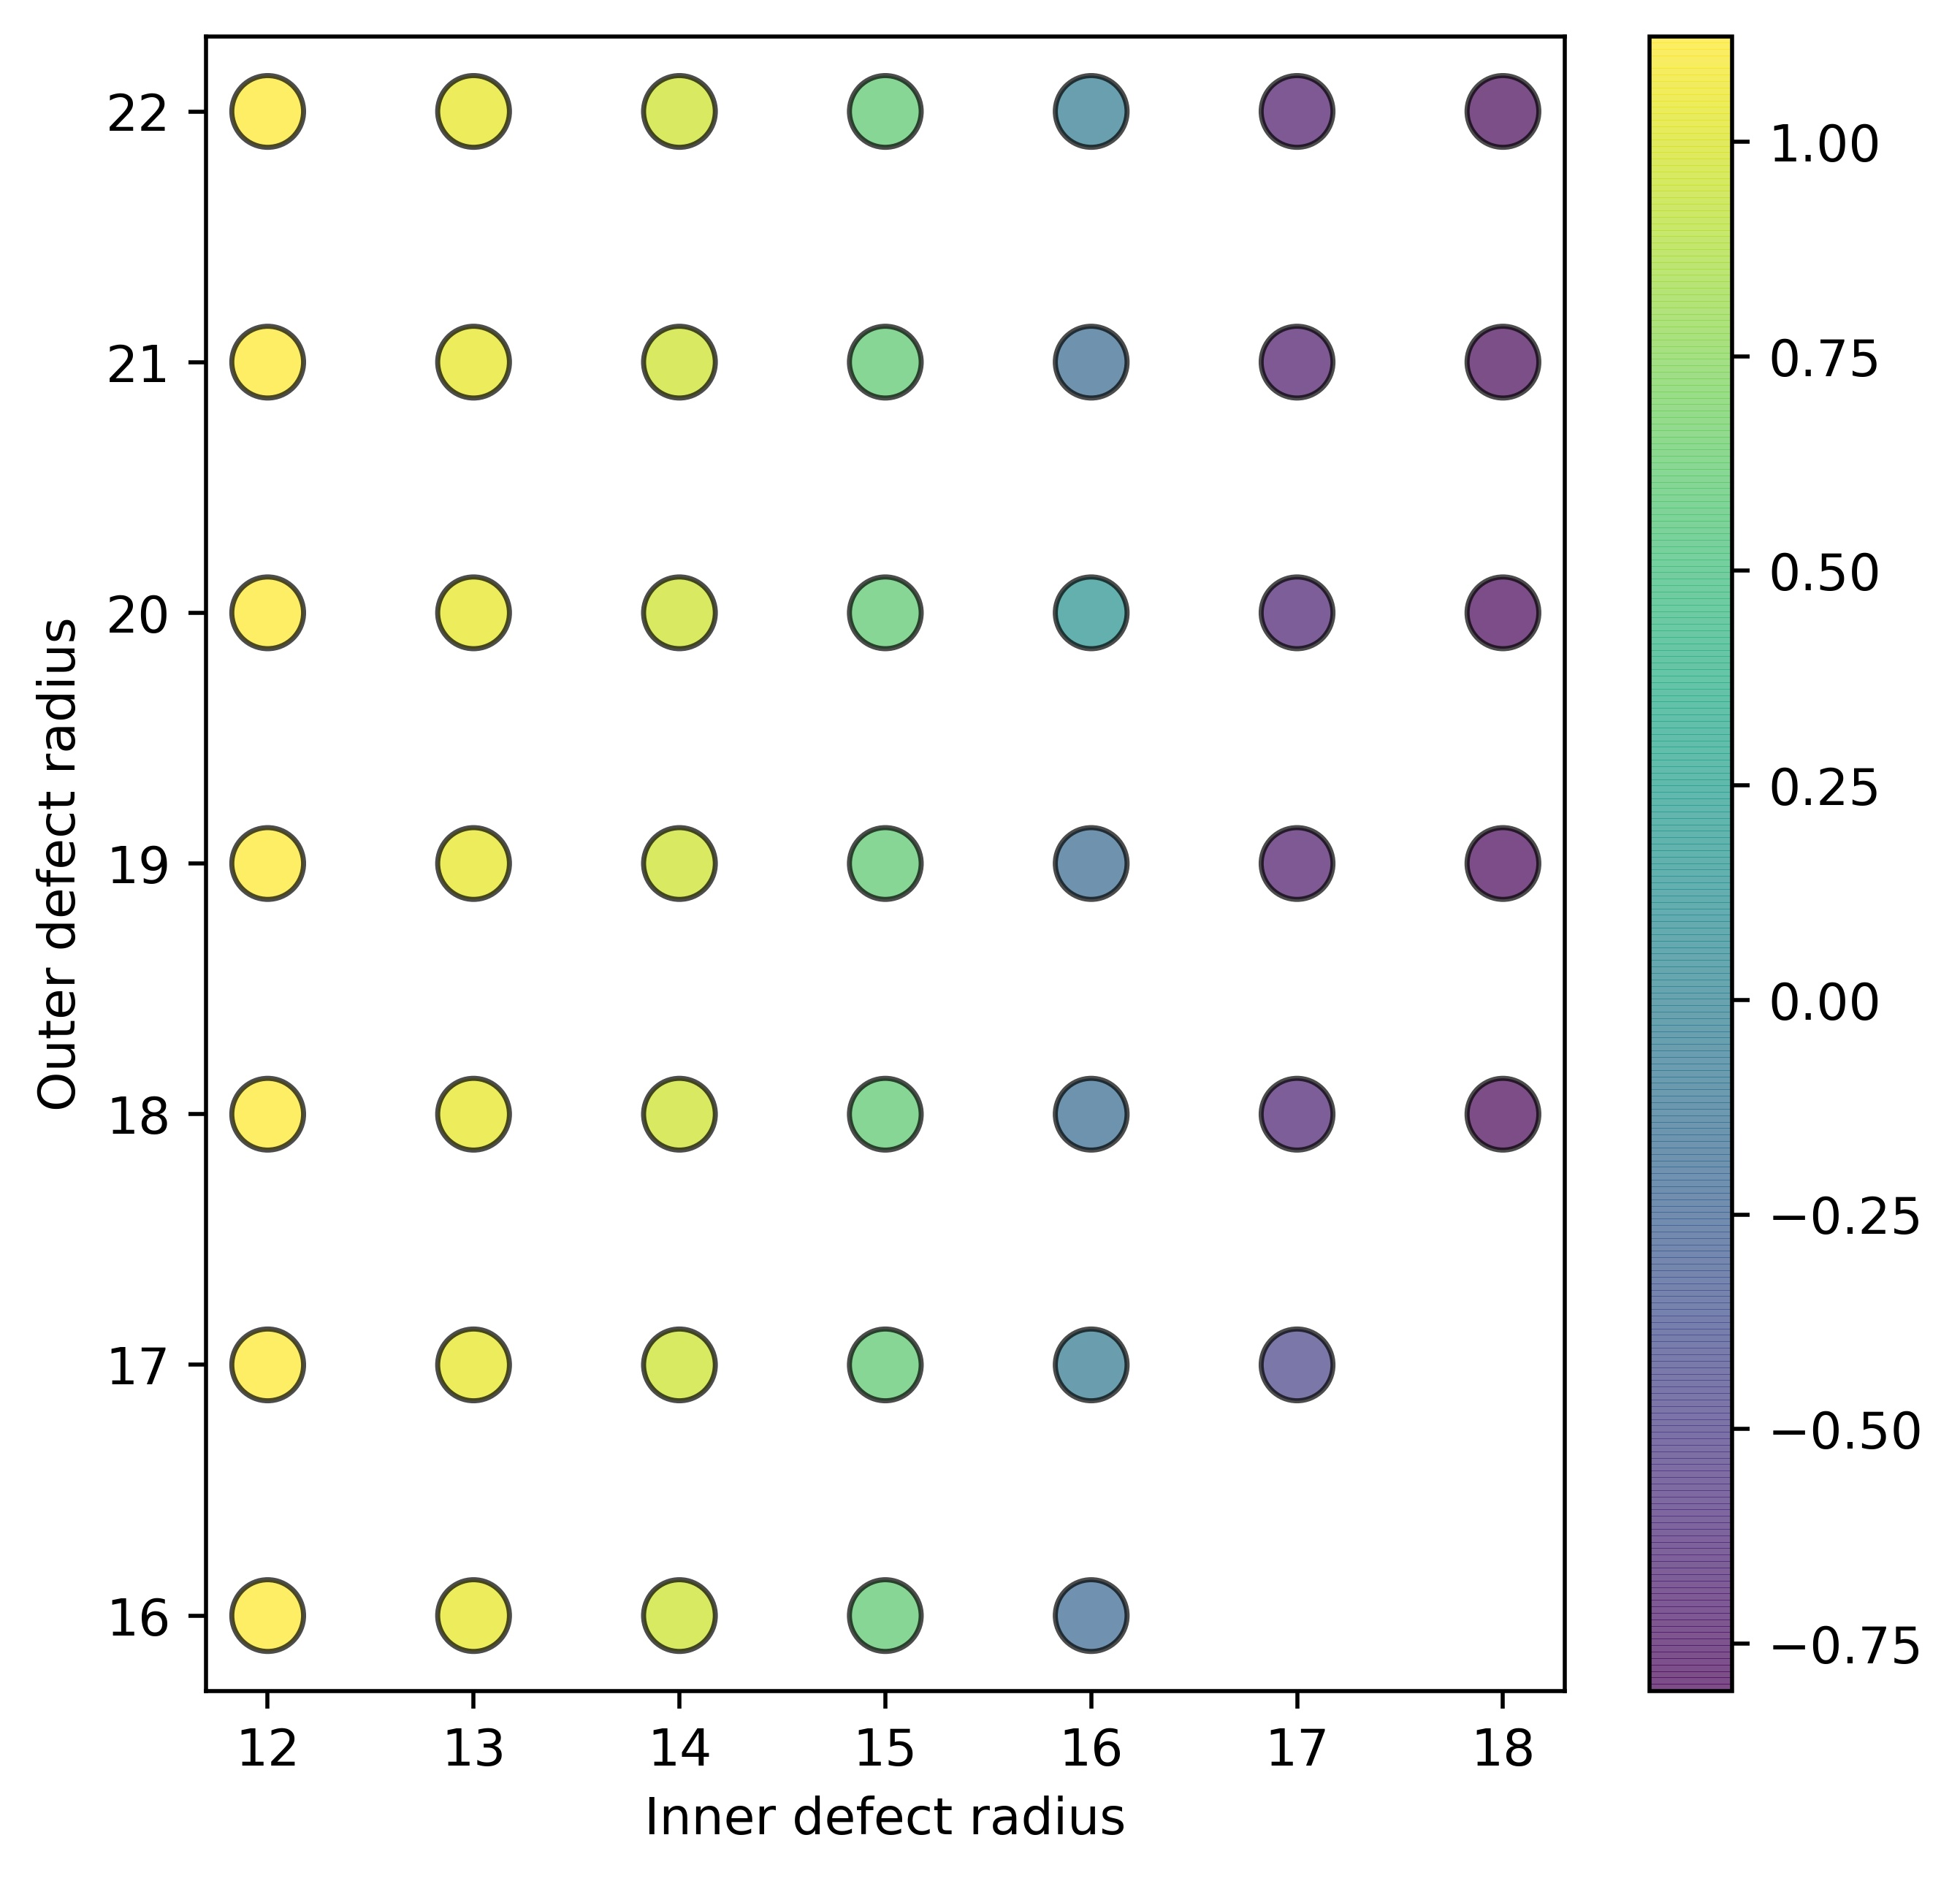
\includegraphics[width=10cm]{na3ocl_namig_defsize.jpg}
\caption{\label{na3ocl_namig_defsize.jpg} The effect of the radius of Region I and Region II in the calculation of the Na migration energy barrier in \ch{Na3OCl} (intersitial fixed in all dimensions)}
\end{figure}

\begin{table}[h!]
  \begin{center}
    \caption{Literature comparison}
    \label{tab:table1}
    \begin{tabular}{l|c|c|c}
      \textbf{Parameter} & \textbf{Calc.} & \textbf{Comp.} & \textbf{Exp.}\\
      \hline
      lattice parameter, $\AA$ & 4.508 & 4.54\cite{RN72}, 4.538\cite{RN78}, 4.382\cite{RN78}, 4.501\cite{RN55} & 4.504\cite{RN53}, 4.496\cite{RN69}, 4.500\cite{RN65}, 4.491\cite{RN68}\\
      Na Frenkel, eV & 1.58 & 1.57\cite{RN72}, 2.6\cite{RN55} & \\
      NaCl Schottky, eV & 1.29 & 1.18\cite{RN72}, 1.8\cite{RN55} & \\
      \ch{Na2O} Schottky, ev & 3.73 & 1.74\cite{RN72} & \\
      \ch{Na3OCl} Schottky, ev & 4.96 & 6.2\cite{RN55} & \\
      Na vacancy migration, eV & 0.68 & 0.61\cite{RN72}, 0.428\cite{RN68}, 0.29\cite{RN53} & 0.63\cite{RN68}, 1.04\cite{RN53} \\
      MgO solution, eV & 2.13 & 1.93\cite{RN72} & \\
      CaO solution, eV & 2.06 & 1.56\cite{RN72} & \\
      SrO solution, eV & 1.32 & 1.28\cite{RN72} & \\
      BaO solution, eV & 1.11 & 0.77\cite{RN72} & \\
      Mg clustering, eV & -0.35 & -0.25\cite{RN72} & \\
      Ca clustering, eV & -0.71 & -0.1\cite{RN72} & \\
      Sr clustering, eV & -0.67 & -0.15\cite{RN72} & \\
      Ba clustering, eV & -1.62 & -0.42\cite{RN72} & \\
    \end{tabular}
  \end{center}
\end{table}

\clearpage

\bibliographystyle{rsc}
\bibliography{/home/ben/Documents/literature_review/exportlist}

\end{document}